% ***** PRÄAMBEL *****
\documentclass[
%  draft,                                                                      %% Entwurf. Entweder dies ODER final
  final,                                                                       %% Final. Entweder dies ODER draft
  12pt,                                                                        %% Schriftgröße
  paper=a4,                                                                    %% Papierformat
  english, ngerman,                                                            %% Sprache(n) des Dokuments (können auch mehrere sein: Auswahl mit \selectlanguage{})
  toc=listof,                                                                  %% Verweis auf Abbildungs- und Tabellenverzeichnisse
  chapterprefix=true,                                                          %% Kapitel beginnen mit "Kapitel NUMMER"
%  twoside,                                                                    %% Zweiseitiger Druck
%  openright,                                                                  %% Kapitelanfänge auf rechter Seite
]{scrreprt}                                                                    %% Dokumentklasse

% ***** Seitenlayout *****
\usepackage[left=3.5cm,right=3cm,top=3cm,bottom=3.5cm]{geometry}               %% Seitenränder   
\setcounter{secnumdepth}{0}                                                    %% Keine Nummerierung von Kapiteln etc.
\usepackage{setspace}                                                          %% Ändern des Zeilenabstands
\setstretch{1.1}                                                               %% Zeilenabstand von 1.1 Punkt

% ***** Kopf- und Fußzeilen *****
\usepackage{scrpage2}                                                          %% Seitenlayout, Fußnoten, Kopf- und Fußzeilen
\pagestyle{scrheadings}                                                        %% Kopfzeilen einstellen
\clearscrheadfoot                                                              %% Kopf und Fußzeilen leeren
\automark{chapter}                                                             %% Kapitelnamen in Kopfzeile
\ohead{\headmark}                                                              %% Kopfzeilentext am äußeren Rand
\setheadsepline{0.4pt}                                                         %% Linie unter dem Kopfzeilentext
\ofoot[\pagemark]{\pagemark}                                                   %% Seitennummern am äußeren Rand

% ***** Laden der Packages *****
\usepackage{mathtools}                                                         %% Mathekrempel für schöne Formeln
\usepackage{graphicx}                                                          %% Grafiken
\usepackage{booktabs}                                                          %% Qualitativ hochwertige horizontale Linien in Tabellen
\usepackage{url}                                                               %% URLs im Text einbinden
\usepackage{textcomp}                                                          %% Verschiedene Symbole und Sonderzeichen
\usepackage{caption}[2008/08/24]                                               %% Unterschriften für Bilder, Tabellen, etc.
\usepackage{babel}                                                             %% Paket für Silbentrennung etc.
\usepackage[T1]{fontenc}                                                       %% Schriftencoding
\usepackage[utf8]{inputenc}                                                    %% Eingabecodierung
\usepackage{lmodern}                                                           %% Schriftart
\usepackage{listings}                                                          %% Erlaubt Syntax-Korrektes Code-Einbinden
\usepackage{color}                                                             %% Farben definieren
\usepackage[svgnames]{xcolor}                                                  %% Vereinfacht den Umgang mit Farben
\usepackage{supertabular}                                                      %% Einfachere Tabellen
\usepackage{scrhack}                                                           %% Hacks, um Pakete mit KOMA-Klassen kompatibel zu machen
\usepackage[pdfborder={0 0 0}, colorlinks=false]{hyperref}                     %% Klickbare Verweise in normaler Textfarbe und ohne Umrandung

% ***** Bibliographie-Setup *****
\usepackage[style=alphabetic-verb, hyperref=auto, backend=biber]{biblatex}   %% Havard-Notation für Naturwissenschaften
\usepackage[babel, german=quotes]{csquotes}                                    %% Deutsche Anführungszeichen
\bibliography{bibliographie/literatur.bib}                                     %% Pfad zur Bibliographiedatei


% ***** DOKUMENT *****
\begin{document}


% ***** TITELSEITE *****
\begin{titlepage}

\begin{center}
%% Upper part of the page
\textsc{\LARGE Beuth Hochschule für Technik}\\
\large{Fachbereich VI - Informatik und Medien\\Studiengang Medieninformatik}\\[50mm]
\textsc{\large Bachelorarbeit}\\
\end{center}
%% Title
\LARGE{\bfseries{Implementierung und Anbindung eines WebGL-Renderers an ein bestehendes Realtime Interactive System}}
\vspace{10mm}

%% Author and supervisor
\begin{center}
\begin{minipage}[t]{0.4\textwidth}
\begin{flushleft} \large
\emph{Autor:}\\
Stefan Reichel
\end{flushleft}
\end{minipage}
\begin{minipage}[t]{0.5\textwidth}
\begin{flushright} \large
\emph{Betreuer:} \\
Stephan Rehfeld (M. Sc.)\\
\medskip
\emph{Zweitbetreuer:} \\
Prof. Dr. Ing. Hartmut Schirmacher
\end{flushright}
\end{minipage}

\vfill

%% Bottom of the page
{\large Tag der Abgabe 03.09.2012}
\end{center}

\end{titlepage}


% ***** ZUSATZ *****
\definecolor{lightgray}{rgb}{.95,.95,.95}
\definecolor{darkgray}{rgb}{.4,.4,.4}
\definecolor{purple}{rgb}{0.65, 0.12, 0.82}

\lstdefinelanguage{JavaScript}{
  keywords={typeof, new, true, false, catch, function, return, null, switch, var, if, in, while, do, else, case, break},
  ndkeywords={class, export, boolean, throw, implements, import, this},
  sensitive=false,
  comment=[l]{//},
  morecomment=[s]{/*}{*/},
  morestring=[b]',
  morestring=[b]"
}

\lstdefinelanguage{Scala}{
  keywords={import, class, object, trait, extends, with, new, if, while, for, def, val, var, this, case, switch, ->, =>},
  sensitive=false,
  comment=[l]{//},
  morecomment=[s]{/*}{*/},
  morestring=[b]"
}
 
\lstset{
  backgroundcolor=\color{lightgray},
  extendedchars=true,
  basicstyle=\footnotesize\ttfamily,
  showstringspaces=false,
  showspaces=false,
  numbers=left,
  numberstyle=\footnotesize,
  numbersep=9pt,
  tabsize=2,
  breaklines=true,
  showtabs=false,
  captionpos=b,
  keywordstyle=\color{blue},
  ndkeywordstyle=\color{darkgray},
  commentstyle=\color{purple},
  stringstyle=\color{red},
  identifierstyle=\color{black}
}


\pagenumbering{roman}


% ***** VERZEICHNISSE *****
\tableofcontents                                                               %% Inhaltsverzeichnis
\listoffigures                                                                 %% Abbildungsverzeichnis
%\listoftables                                                                 %% Tabellenverzeichnis
\lstlistoflistings                                                             %% Listingverzeichnis

\addcontentsline{toc}{chapter}{Listings}                                       %% Referenz auf Listingverzeichnis im Inhaltsverzeichnis


% ***** INHALT *****
\addchap{Vorwort}
\label{chap:vorwort}
Schon vor meinem Studium beschäftigte ich mich mit den Möglichkeiten moderner 3D-Grafik. Ich erstellte Modifikationen für Computerspiele, wie neue, höher auflösende Texturen, durch die sich die visuelle Qualität deutlich steigern ließ. Durch das Studium lernte ich die technischen Aspekte kennen und experimentierte mit eigenen kleinen Anwendungen in OpenGL und WebGL. Daher war mir klar, dass ich in meiner Bachelorarbeit gern tiefer in dieses Thema einsteigen würde. Der Betreuer dieser Arbeit, Herr Stephan Rehfeld, brachte mich auf die Idee das Thema WebGL mit der Anbindung an ein Realtime Interactive System (RIS) zu kombinieren. Die Beuth Hochschule hat in den letzten Jahren in Kooperation mit der Universität Würzburg ein neuartiges RIS entwickelt, welches auch bereits auf dem "`Holodeck"' der Beuth Hochschule verwendet wird. Herr Rehfeld ist Teil dieses Teams, wodurch ich bei Fragen zum System schnelle und präzise Antworten bekam. Danke dafür noch einmal an ihn.

Solch ein RIS könnte komplexe Berechnungen wie die Physik übernehmen und den clientseitigen Renderer so entlasten. Auf diese Weise wäre es möglich sehr ressourcenintensive 3D-Anwendungen im Browser auch schwächerer Clients auszuführen. Dies wird in Zukunft von größerer Relevanz sein, da die derzeitige Entwicklung weg von starren Desktop-Computern und hin zu mobilen Clients, wie Notebooks, Netbooks, Smartphones und Tablets geht. Diese Endgeräte sind mittlerweile zwar sehr leistungsstark, jedoch für aufwendige 3D-Anwendungen noch immer nur begrenzt einsetzbar und es muss für jede Plattform eine eigene Clientanwendung geschrieben werden. Über nativ im Browser ausgeführtes WebGL und ein auf einem Server laufendes RIS tun sich jedoch auch hier neue Möglichkeiten für eine komplexe Echtzeitdarstellung auf.


\clearpage
\pagenumbering{arabic}

\chapter{Einführung}
\label{chap:einführung}
\nocite{*}

\section{Motivation}
\label{sec:motivation}
Immer mehr Anwendungen werden in das Internet verlagert. Zugriff darauf erlangt man in der Regel über den Browser. Dies hat enorme Vorteile sowohl für Entwickler und Unternehmen als auch die Anwender selbst. So können sich die Entwickler in der Regel auf eine Entwicklungsumgebung (HTML, CSS und JavaScript) konzentrieren und müssen keine plattformspezifischen Lösungen finden. Die Anwender benötigen nur einen modernen und standardkonformen Browser um die Anwendungen nutzen zu können. Mit HTML5 ist auch ein neuer Standard in der Entwicklung der selbst viele neue Möglichkeiten für Entwickler bringt (Canvas-Element, Geolocation-API, File-API etc.) und in dessen Umfeld ebenso neue Standards entstehen, mit denen sich Anwendungen realisieren lassen die früher schlichtweg so nicht denkbar waren.

3D-Anwendungen wie Computerspiele oder CAD-Werkzeuge konnten bisher allerdings je nach Komplexität gar nicht oder nur über Drittanbieterlösungen (zum Beispiel Adobe Flash) im Browser angeboten werden. Ein neuer Standard aus dem Umfeld von HTML5 könnte die Situation jedoch stark verbessern: WebGL. WebGL ermöglicht es Entwicklern komplexe 3D-Anwendungen in Echtzeit ohne Plugins oder sonstige externe Lösungen nativ im Browser auszuführen. Die Berechnung der Inhalte erfolgt direkt auf der Grafikhardware des Clients und ermöglicht somit auch detailreiche und ressourcenintensive Darstellungen.

\section{Zielsetzung}
\label{sec:zielsetzung}
Den Rahmen dieser Arbeit bildet eine Anwendungsexploration eines vernetzten 3D-Echtzeit-Renderingsystems, welches eine vordefinierte 3D-Szene darstellen und der Anwender darin enthaltene Entitäten per Tastendruck manipulieren kann. Das grafische Rendering der Szene wird von einem komplett selbst implementierten WebGL-Renderer übernommen, die Berechnung der Physik von einer ebenfalls an ein Realtime Interactive System angebundenen Physikengine. Das komplette System wird aus drei Komponenten bestehen:
\begin{itemize}
    \item \textbf{WebGL-Renderer}\\
Der Renderer wird vollständig neu in JavaScript implementiert und im Browser des Clients ausgeführt. Er kommuniziert über ein WebSocket in Echtzeit mit dem Server.
    \item \textbf{Webserver}\\
Der Webserver stellt die benötigten Ressourcen (z.B. HTML-Seiten, Szenen, 3D-Modelle und Texturen) für den Client bereit und ist die zentrale Schnittstelle für die Kommunikation zwischen Client und RIS. Das heißt, dass der Server in Echtzeit Nachrichten vom Client empfängt, in ein für das RIS verständliches Format umwandelt und an dieses weiterleitet. Das gleiche gilt in entgegengesetzter Richtung für Nachrichten vom RIS an den Client.\\
Als Plattform habe ich mich für das Play! Framework entschieden (siehe Abschnitt \textit{Konzeption}).
    \item \textbf{Realtime Interactive System}\\
Als RIS werde ich SIRIS verwenden. SIRIS enthält in der derzeit aktuellen Version die JBullet-Physikengine\footnote{\url{http://jbullet.advel.cz} (besucht am \today)}, welche die physikalischen Kräfte auf die Objekte in der Szene berechnen wird. SIRIS abstrahiert den Zugriff auf sie völlig, weshalb ich auch nicht näher auf sie eingehen werde. Zudem ist es möglich dass sie in Zukunft durch eine andere Physikengine ersetzt wird.

Da SIRIS in Scala implementiert ist und das Play! Framework diese Programmiersprache ebenfalls anbietet werde ich die Anbindung des Renderers ebenfalls in Scala vornehmen.
\end{itemize}
Das komplette System wird Prototypenstatus haben. Zum Einen, da es im Zuge einer Bachelorarbeit mit ihrem eng gefassten Zeitrahmen nur schwerlich möglich ist sich allein in alle benötigten Themenfelder einzuarbeiten und ein "`vollständiges"' System aufzubauen. Zum Anderen sind die verwendeten Technologien noch relativ neu und es gibt nur wenige akademisch verwertbare Referenzen an denen man sich, beispielsweise für die Systemarchitektur, orientieren kann.

\chapter{Verwendete Technologien}
\label{chap:technologien}

\section{WebGL}
\label{sec:webgl}
3D-Szenen im Webbrowser darzustellen wurde 1997 zuerst von den Ingenieuren von SGI (Silicon Graphics Incorporated) versucht \autocite[110]{Zielgerichtet}. Die damaligen Heimcomputer waren dafür aber hardwaremäßig viel zu schwach ausgestattet, sodass die Anwendungen hauptsächlich auf teuren dedizierten Workstations liefen. Dennoch wurde der Ansatz weiterverfolgt und ein Konsortium entwickelte den ISO-Standard VRML97. Dieser war jedoch für Entwickler schwer zu handhaben und ließ sich nicht gut in die Webseite integrieren. Daher fand er nur eine geringe Verbreitung. Das Konsortium entwickelte die Idee jedoch weiter und veröffentlichte X3D\footnote{\url{http://www.web3d.org/realtime-3d/x3d/what-x3d/} (besucht am \today)}, ein XML-basiertes Beschreibungsformat für 3D-Szenen. Auch dieses blieb aber eine Nischenlösung.

Einen wirklichen Durchbruch für interaktive 3D-Inhalte im Webbroswer könnte WebGL bringen, welches von den meisten modernen Browsern bereits vollumfänglich unterstützt wird (auch wenn die Unterstützung häufig noch als experimentell deklariert ist). Es lässt sich in den folgenden Browsern verwenden:
\begin{itemize}
    \item Google Chrome ab Version 9
    \item Mozilla Firefox ab Version 4
    \item Safari ab Version 5.1 (muss manuell aktiviert werden)
    \item Opera ab Version 11
\end{itemize}
Microsoft hat derzeit noch keine Pläne angekündigt WebGL in den Internet Explorer zu integrieren.

WebGL ist ein Application Programming Interface (API) basierend auf OpenGL ES 2.0, dem OpenGL-Standard für mobile Endgeräte \autocite{OpenGlES}, und wird von der Khronos Group aktiv entwickelt. Die Khronos Group ist ein Non Profit-Konsortium das sich mit der Entwicklung von Standards für Computergrafik, nebenläufige Programmierung, dynamische Medien und andere Themenfelder befasst. Die Spezifikation für die Version 1.0 ist im Februar 2011 erschienen \autocite{WebGLSpec}. Es basiert zwar auf OpenGL ES 2.0, allerdings gibt es einige kleine Unterschiede deren man sich gewahr sein muss wenn man aus dem OpenGL ES-Umfeld kommt (siehe \autocite{WebGLDiff}). Für die Programmierung wird JavaScript direkt verwendet oder eine Sprache die nach JavaScript kompiliert (beispielsweise CoffeeScript\footnote{\url{http://coffeescript.org} (besucht am 16. August 2012)} oder Dart\footnote{\url{http://www.dartlang.org} (besucht am 16. August 2012)}). Die Grundlage für das Zeichnen in WebGL ist das HTML5-Element \textit{canvas}. Aus diesem Grund wird WebGL auch häufig zum HTML5-Standard dazugezählt, ist aber bis auf die Abhängigkeit vom Canvas-Elements völlig eigenständig.

Eine WebGL-Anwendung besteht, wie die meisten Webanwendungen, aus HTML-Seiten, JavaScript- sowie CSS-Dateien und wird in einem Webbrowser ausgeführt. Im Gegensatz zu den herkömmlichen Methoden 3D im Browser darzustellen (X3D, Flash, etc.) hat WebGL den großen Vorteil, dass kein spezielles Plugin benötigt wird. Die Unterstützung ist nativ in die Browser eingebaut. Informationen über die darzustellenden Inhalte sowie die Art und Weise wie diese dargestellt werden, werden über JavaScript direkt an die WebGL-API weitergegeben. Zu diesen Informationen gehört neben den darzustellenden Inhalten auch WebGL-spezifischer Inhalt, wie der Code für die verwendeten Shader.
\begin{figure}
\centering
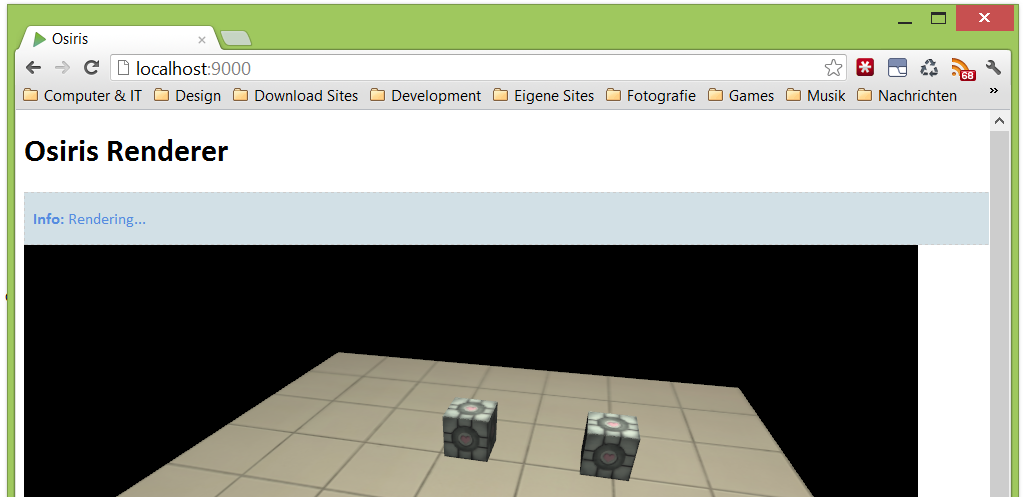
\includegraphics[width=\textwidth]{bilder/canvas.png}
\caption{3D-Szene gerendert im Canvas mit WebGL}
\label{fig:webglcanvas}
\end{figure}
\begin{figure}
\centering
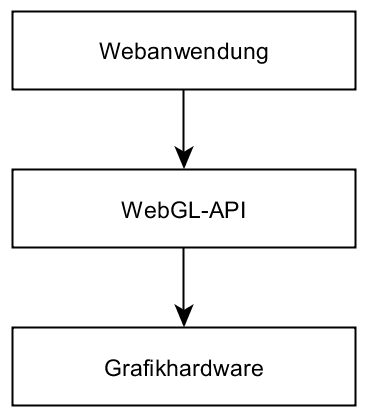
\includegraphics[height=50mm]{bilder/webglflow.png}
\caption{Befehlsfluss in einer WebGL-Anwendung}
\label{fig:webglflow}
\end{figure}
In den folgenden Abschnitten werde ich die wichtigsten Elemente vorstellen, die für das Verstehen einer WebGL-Anwendung unerlässlich sind.

\subsection{Der Kontext}
Das HTML5-Canvaselement stellt verschiedene Kontexte bereit, über die man den dargestellten Inhalt manipulieren kann. Der WebGL-Kontext hat, je nach Browserhersteller, derzeit noch verschiedene Namen. Allerdings soll dies zukünftig auf "`webgl"' standardisiert werden. Mit Hilfe der Bibliothek \textit{WebGLUtils}\footnote{\url{https://cvs.khronos.org/svn/repos/registry/trunk/public/webgl/sdk/demos/common/webgl-utils.js} (besucht am 16. August 2012)} von Google reicht allerdings ein einzelner Funktionsaufruf.

Der WebGL-Kontext enthält alle Funktionsaufrufe an die WebGL-API und ist somit die direkte Verbindung zur Grafikhardware des Computers. Daher ist er an sehr vielen Stellen innerhalb der Anwendung von enormer Bedeutung.

Durch verschiedene Ereignisse kann der Kontext verloren gehen. Die Grafikhardware ist eine geteilte Ressource und kann plötzlich von anderen Prozessen in Anspruch genommen werden oder eine WebGL-Anwendung erzeugt einen Timeout, wodurch der Grafikkartentreiber die Hardware zurücksetzt. Es gibt viele Gründe warum der Kontext verloren gehen kann. Wichtig ist nur zu verstehen, dass es jederzeit passieren kann, wodurch die Anwendung dann nicht mehr funktionieren wird. Daher muss unbedingt darauf geachtet werden, dass eine WebGL-Anwendung auf den Kontextverlust angemessen reagiert. Das Canvas-Element bietet hierfür zum einen die Möglichkeit zwei Eventlistener zu registrieren. Ein Eventlistener reagiert auf das \textit{webglcontextlost}-Event was, wie der Name schon sagt, ausgelöst wird sobald der Kontext verloren geht. Der zweite Eventlistener reagiert auf \textit{webglcontextrestored} und zeigt an, dass der Kontext wiederhergestellt wurde. Zum anderen ist es möglich über die Funktion \texttt{isContextLost} jederzeit den Zustand des Kontexts abzufragen.

\subsection{Shader}
Wie OpenGL ES 2.0 ist auch WebGL rein shaderbasiert. Shader sind kleine Programme die die eingehenden Informationen (3d-Modelldaten, Texturen, Beleuchtung etc.) verarbeiten und, je nach programmiertem Verhalten, bestimmen was letztendlich auf dem Canvas zu sehen sein wird. Sie werden direkt auf der Grafikhardware ausgeführt und erlauben somit eine sehr flexible und performante Darstellung der Szene.

In WebGL ist man auf zwei Shadertypen beschränkt: den Vertex- und den Fragmentshader. Diese werden in der OpenGL ES Shading Language (GLSL ES) geschrieben und müssen vor Gebrauch kompiliert und zu einem Shaderprogramm verbunden werden. Auch hierfür ist kein externer Compiler nötig. Dieser wird vom Grafikkartentreiber bereitgestellt und der Vorgang wird direkt vom Browser über JavaScript-Funktionsaufrufe der WebGL-API angestoßen (siehe Listing \ref{lst:createshaderfromsource}).
\lstset{language=JavaScript}
\begin{lstlisting}[caption={Erstellen eines Shaders (selbstgeschriebene Funktion)}, label={lst:createshaderfromsource}]
function createShaderFromSource(type, source) {
  var glShader = gl.createShader(type);
  gl.shaderSource(glShader, source);
  gl.compileShader(glShader);

  return glShader;
}
\end{lstlisting}
Der Shadercode muss als String an die Funktion \texttt{shaderSource} übergeben werden. Dies ist sehr flexibel, da man den Code so auf viele Arten in die Anwendung einbringen kann. So kann er beispielsweise in die HTML-Seite eingebunden oder direkt im JavaScript-Code festgelegt werden.

\subsection{Shaderaufbau}
Der Vertex- und Fragmentshader haben einen ähnlichen Aufbau. Zu Beginn müssen alle eingehenden und ausgehenden (nur Vertexshader) benutzerdefinierten Daten mit ihren Typen deklariert werden. Von der API können jedem der beiden Shader benutzerdefinierte \textit{Uniforms} mitgegeben werden. Uniforms sind Daten, die für alle Vertices\footnote{Ein Vertex ist ein Eckpunkt eines 3D-Modells.} pro Zeichnungsaufruf konstant bleiben, wie die Positionen und Farben von Lichtquellen oder Transformationsmatrizen.

Die GLSL ES ist eine an C angelehnte Sprache und bietet einen ausreichenden Satz von Features. Eigene Variablen können verwendet, in Structs zusammengefasst und Shaderlogik in Funktionen untergebracht werden. Zudem gibt es eine den meisten Programmierern wohlvertraute \texttt{main}-Funktion, innerhalb derer das Hauptprogramm abläuft. Die Hauptaufgabe eines Shaders ist es, "`seine"' spezielle globale Variable zu befüllen.

\subsubsection{Vertexshader}
Der Vertexshader hat die alleinige Aufgabe die 3D-Modelldaten (genauer: die Vertices) innerhalb der Szene zu manipulieren, d.h. in seinem Quelltext muss die globale Variable \texttt{gl\_Position} befüllt werden. Er wird immer zuerst ausgeführt und kann Berechnungsergebnisse (bsp. Normalentransformationen) an den Fragmentshader weitergeben. Dies geschieht über sogenannte \textit{Varyings}. Varyings sind von außen nicht zugreifbar. Zusätzlich zu den Uniforms können ihm pro Zeichenaufruf für jedes Vertex veränderliche Daten über \textit{Attributes} mitgeteilt werden. Dies sind beispielsweise die Position, die Normale, die Farbe etc.
\begin{figure}
\centering
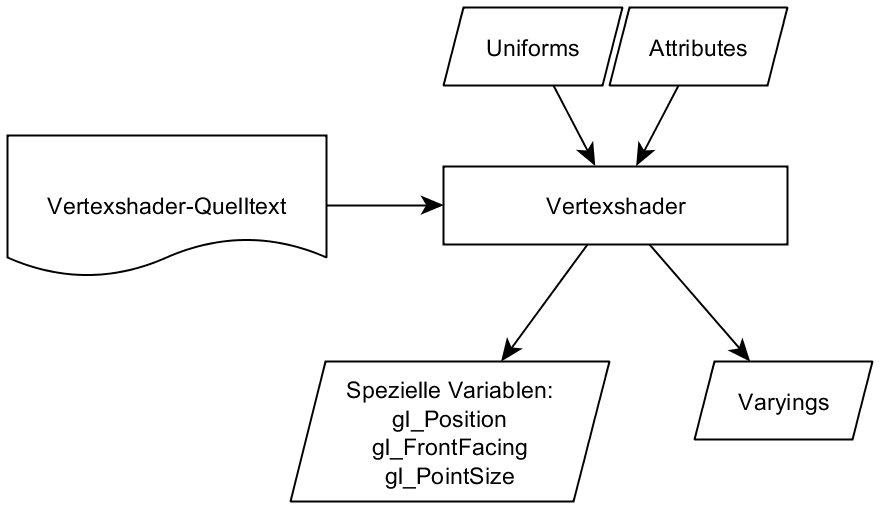
\includegraphics[height=60mm]{bilder/vertexshader.png}
\caption{Datenfluss in den und aus dem Vertexshader, nach \autocite{WebGlPogramming}}
\label{fig:vertexshader}
\end{figure}

\subsubsection{Fragmentshader}
Der Fragmentshader legt die Farbe eines Fragments\footnote{Ein Fragment entspricht einem Pixel auf dem Bildschirm, allerdings können in den nachfolgenden Fragmentoperationen der Rendering Pipeline einige Fragmente auch wieder verworfen werden. Daher die Unterscheidung zwischen Fragment und Pixel.} fest, d.h. in seinem Quelltext muss die globale Variable \texttt{gl\_FragColor} befüllt werden.

Neben den Uniforms und Varyings können dem Fragmentshader \textit{Sampler} übermittelt werden. Dies sind spezielle Uniforms, die für die Texturierung verwendet werden.

Am Anfang des Fragmentshader-Codes muss zwingend die Mindestpräzision für alle Fließkommaoperationen angegeben werden. In der Regel nutzt man hierfür die in Listing \ref{lst:fragmentshaderprecision} dargestellte Zeile.
\lstset{language=C}
\begin{lstlisting}[caption={Festlegen der Mindestpräzision für alle Fließkommaoperationen}, label={lst:fragmentshaderprecision}]
precision mediump float;
\end{lstlisting}
Dies ist vor allem für Anwendungen wichtig, bei denen die visuelle Qualität stark von der Genauigkeit der (unter Umständen sehr komplexen) Berechnungen abhängt. Allerdings kann die Wahl (\texttt{lowp}, \texttt{mediump} oder \texttt{highp}) auch Auswirkungen auf die Leistung haben oder wird von manchen Geräten (insbesondere im Mobilbereich) nicht unterstützt \autocite{WebGlPrecision}. Daher ist es ratsam immer entweder \texttt{lowp} oder \texttt{mediump} zu verwenden, je nach Anwendungsfall.
\begin{figure}
\centering
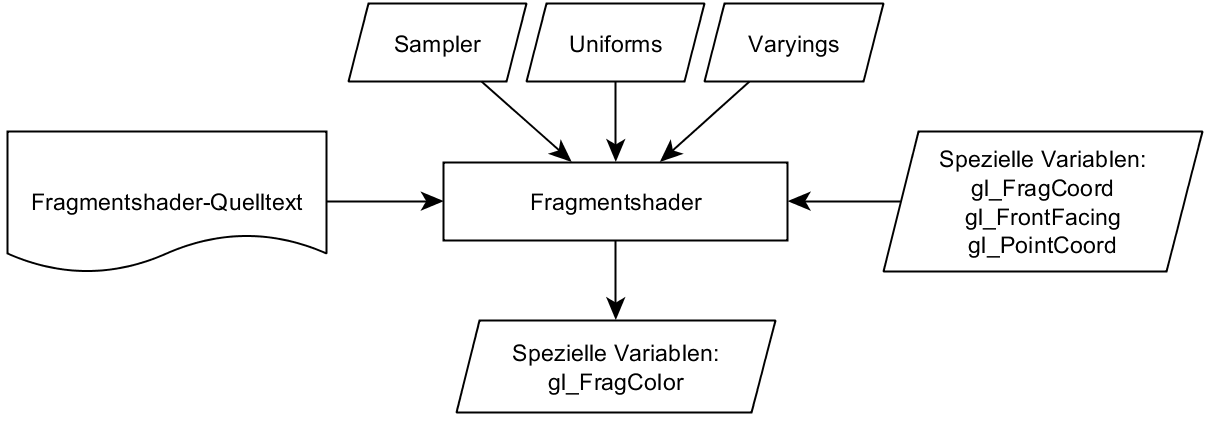
\includegraphics[width=\textwidth]{bilder/fragmentshader.png}
\caption{Datenfluss in den und aus dem Fragmentshader, nach \autocite{WebGlPogramming}}
\label{fig:fragmentshader}
\end{figure}

\subsection{Drawing Buffer}
Grafikkarten verfügen über einen Framebuffer in dem die Bilder (Frames), die später auf dem Monitor zu sehen sein werden, zusammengebaut werden. WebGL hat eine eigene Art von Framebuffer, den \textit{Drawing Buffer}. Wenn ein Renderzyklus erfolgreich abgeschlossen wurde und alle Daten die WebGL-Pipeline durchlaufen haben, wird aus ihnen im Drawing Buffer das fertige Bild erstellt. Dieses wird jedoch nicht direkt auf dem Monitor dargestellt, sondern mit dem Rest der HTML-Seite verbunden und dann an den Framebuffer der Grafikkarte gesendet. Dieser sendet es letztendlich an den Monitor \autocite[5--7]{WebGlPogramming}.

\section{WebSockets}
\label{sec:websockets}
Browser kommunizieren mit Servern über das Hypertext Transfer Protocol (HTTP). HTTP ist völlig statuslos und funktioniert nach dem Muster Request $\rightarrow$ Response. Alle Kommunikation geht hierbei vom Client aus, der eine Anfrage (Request) an den Server schickt. Dieser verarbeitet die Anfrage und sendet dem Client eine Antwort (Response). Hiernach schließt er die Verbindung und der Vorgang ist abgeschlossen. Dieses Verfahren ist für Echtzeit-Anwendungen jedoch aus folgenden Gründen problematisch:
\begin{itemize}
    \item HTTP erzeugt unnötigen Overhead \autocite[673]{WebsocketsFurukawa}. Da die Kommunikation statuslos ist werden bei jeder Anfrage viele Informationen mitgeschickt die für die eigentlich Aufgabe nicht benötigt werden, wie Header- und Statusinformationen. Dadurch ist der Server mit dem unnötigem Abarbeiten der immer gleichen und zu großen Informationspakete beschäftigt und kann so nicht seine volle Kapazität den anstehenden Berechnungen für den Client widmen. Zudem wird für jeden neuen Request eine komplett eigenständige HTTP-Verbindung in Gang gesetzt.
    \item Die Kommunikation ist unidirektional \autocite{WebsocketsRichter}. Da alle Kommunikation vom Client initiiert wird, hat der Server keine Möglichkeit den Client zu benachrichtigen sobald sich serverseitig Daten geändert haben. Erst bei der nächsten Anfrage würden die geänderten Daten geschickt werden. In einem Echtzeitsystem müsste der Client also den Server permanent anfragen (Pollen), was jedoch sowohl den Client als auch den Server unnötig belastet.
\end{itemize}
\begin{figure}
\centering
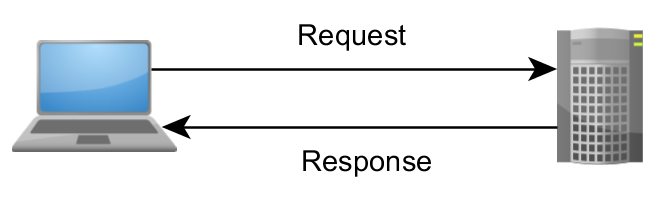
\includegraphics[width=80mm]{bilder/http.png}
\caption{Request/Response-Prinzip des HTTP-Protokolls}
\label{fig:http}
\end{figure}
Um das Problem der unidirektionalen Kommunikation teilweise zu lösen wurde das \textit{Comet}-Anwendungsmodell entworfen. Normalerweise sendet der Server bei unveränderten Daten eine leere Antwort und schließt dann die Verbindung. Ein Comet-Server lässt die Verbindung bei unveränderten Informationen zum Client jedoch so lange offen, bis neue Informationen da sind und sendet erst dann eine Antwort. Allerdings kann der Client keine neuen Informationen senden solange der vorige Request noch nicht beantwortet wurde und es wird immer noch für jeden Request eine eigene Verbindung aufgebaut \autocite[673]{WebsocketsFurukawa}.

In vielen Programmiersprachen wie Java, C/C++ oder C\# stehen dem Programmierer Konstruktionen für den Aufbau einer direkten TCP-Verbindung zum Server bereit. In JavaScript fehlte dies aufgrund der Beschränkung des Browsers auf HTTP bisher. Mit dem WebSocket API-Standard, der sich noch in der Entwicklung befindet (siehe \autocite{WebSocketApiSpec}), wird dieser Missstand jedoch zumindest teilweise behoben. Teilweise, da WebSockets immer auf der Anwendungsebene (Ebene 7) des ISO-OSI-Modells arbeiten \autocite{WebsocketsRichter} und so keine "`echten"' low-level Binärsockets darstellen. Der aktuelle Stand der Protokollspezifikation \autocite{WebSocketRFC} wird von folgenden Browsern unterstützt:
\begin{itemize}
    \item Google Chrome ab Version 16
    \item Mozilla Firefox ab Version 11
    \item Safari ab Version 6
    \item Internet Explorer ab Version 10
    \item Opera ab Version 12.50 (Entwicklerversion)
\end{itemize}
Aus der obigen Liste ist ersichtlich, dass für WebSockets ein noch aktuellerer Browser benötigt wird als für WebGL.

\subsection{Verbindungsaufbau}
Eine WebSocket-Verbindung startet immer als regulärer HTTP-Request. Dieser muss jedoch an eine Adresse gehen, die mit \textit{"`ws:\textbackslash\textbackslash"'} beginnt, statt mit \textit{"`http:\textbackslash\textbackslash"'}. Weiterhin muss der angesprochene Server das WebSocket-Protokoll auch unterstützen. Hiervon gibt es mittlerweile einige für unterschiedliche Programmiersprachen, wie die aktuellen Versionen der Jetty\footnote{\url{http://www.eclipse.org/jetty} (besucht am 17. August 2012)} und Glassfish\footnote{\url{http://www.oracle.com/technetwork/java/javaee/overview/index.html} (besucht am 17. August 2012)}-Server für Java oder PyWebsocket\footnote{\url{http://code.google.com/p/pywebsocket} (besucht am 17. August 2012)} für Python.\\
Ein WebSocket in der Clientanwendung zu initialisieren ist sehr leicht, wie Listing \ref{lst:websocketinit} zeigt.
\lstset{language=JavaScript}
\begin{lstlisting}[caption={Initialisieren einer WebSocket-Verbindung im Browser}, label={lst:websocketinit}]
var socket = new WebSocket("ws://HOST:PORT");

socket.onmessage = function(event) {
  // handle incoming messages
};

socket.onerror = function(error) {
  // handle errors with the connection
};

socket.onopen = function() {
  // the connection to the server has been establishes successfully
};

socket.onclose = function() {
  // the connection has been closed
};
\end{lstlisting}
Wie man sieht ist ein WebSocket über Callbacks eventgesteuert.

Das Socket sendet nun einen \textit{Upgrade}-Request inklusive einiger Zusatzinformationen (siehe \autocite{WebsocketsRichter}) als HTTP-Request an den WebSocket-Server. Wenn dieser die Verbindung annimmt, sendet er eine HTTP-Response und die Verbindung wird auf eine Full-Duplex\footnote{Gleichzeitiger Datenaustausch in beide Richtungen möglich} WebSocket-Verbindung aktualisert. Hierdurch wird das \textit{open}-Event ausgelöst und es können nun in Echtzeit Daten vom Client an den Server, sowie vice versa gesendet werden.
\begin{figure}
\centering
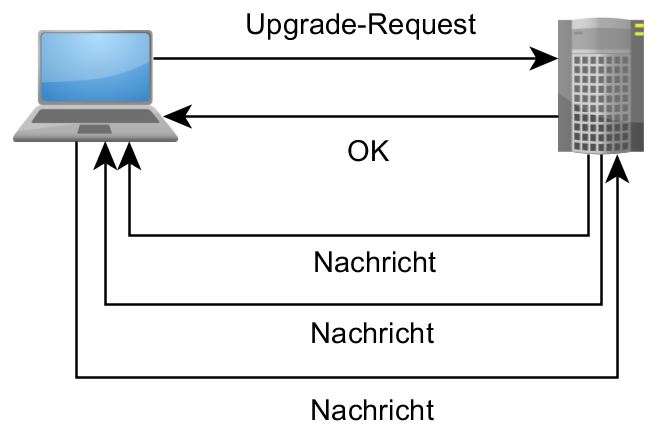
\includegraphics[width=80mm]{bilder/websocket.png}
\caption{Kommunikationsprinzip des WebSocket-Protokolls}
\label{fig:websocket}
\end{figure}

\subsection{Senden und Empfangen}
Sobald das \textit{open}-Event empfangen und somit das für \texttt{onopen} registrierte Callback ausgeführt wurde, lassen sich über die Methode \texttt{send} Daten als Strings an den Server schicken. Der Server kann von sich aus jederzeit Daten senden, wodurch das \textit{message}-Event ausgelöst und damit das für \texttt{onmessage} registrierte Callback aufgerufen wird. Über den \texttt{event}-Parameter des Callbacks lässt sich die Property \texttt{event.data} auslesen, welche die Nachricht des Servers als String beinhaltet.

\section{Realtime Interactive System}
\label{sec:ris}
Ein Realtime Interactive System (kurz RIS) ist ein System mit dem man in Echtzeit interagieren kann, welches also Eingaben sofort verarbeitet und die Ergebnisse zurückliefert. Das prominenteste Beispiel (und ein Spezialfall) hierfür sind wohl Computerspiele. In einem RIS werden in aller Regel verschiedenartige Komponenten miteinander verbunden wie eine 3D-Engine, eine Physik-Engine, eine AI-Engine\footnote{Artifical Intelligence (Künstliche Intelligenz)} und möglicherweise noch einige mehr. Drei für ein RIS typische Architekturmerkmale sind ein Szenengraph, ein Eventsystem und ein Entitymodell \autocite[299]{GuruMeditation}. Das RIS kümmert sich dann unter anderem darum, dass die Komponenten miteinander kommunizieren können. Dies ist wichtig, da beispielsweise die 3D-Engine die Transformationsdaten für die dargestellten Objekte von der Physik erhalten und der Handler für Tastatur- und Mauseingaben der Physik mitteilen können muss, welches Objekt gerade vom Benutzer manipuliert wird. Bei der Entwicklung arbeiten häufig verschieden spezialisierte Teams an den einzelnen Komponenten. So wird die 3D-Engine von Grafikprogrammierern, die AI-Engine von AI-Programmierern entwickelt. Schon am Anfang stellt sich für alle Teams das Problem die Programmierschnittstelle der eigenen Komponente für andere Komponenten zu definieren. Da sich die Ein- und Ausgabedaten in der Regel unterscheiden ist es oft mit erheblichem Aufwand verbunden im Nachhinein eine Komponente gegen eine andere auszutauschen. Im Folgenden werden einige relevante Dinge zu SIRIS erläutert, dem für diese Arbeit gewählten RIS.

\subsection{SIRIS}
SIRIS (Semantic Reflection for Intelligent Realtime Interactive Systems) ist ein Framework mit dem sich komponentenbasierte RIS bauen lassen. Es ist eine noch in der Entwicklung befindliche Gemeinschaftsarbeit zwischen der Beuth Hochschule für Technik Berlin und der Universität Würzburg. Die Dokumentation des Systems ist allerdings noch äußerst spärlich.
\begin{figure}
\centering
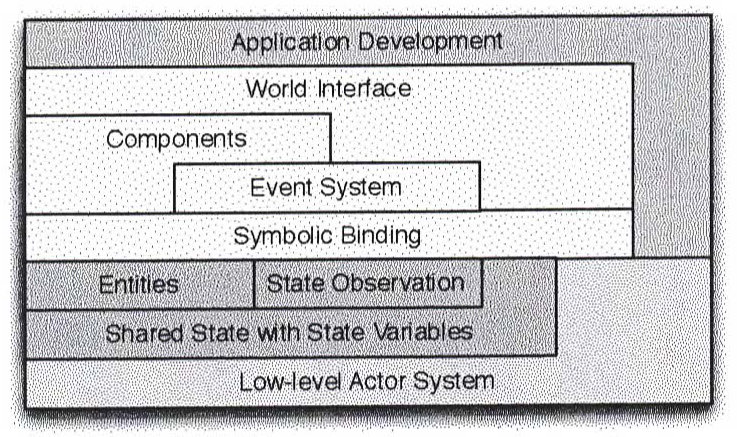
\includegraphics[width=90mm]{bilder/siris_arch.png}
\caption{Systemstruktur von SIRIS \autocite{SimulatorX}}
\label{fig:sirisarch}
\end{figure}

Die funktionalen Komponenten sind in SIRIS stark voneinander entkoppelt, da alle Kommunikation über eine einheitliche Schnittstelle, das \textit{World Interface}, läuft. Das World Interface hat hierbei vier Aufgaben (zitiert nach \autocite[48]{WorldInterface}):
\begin{enumerate}
    \item Benachrichtigung über Änderungsereignisse relevanter Simulationszustände
    \item Ausführen von Aktionen zur Änderung relevanter Simulationszustände
    \item Verarbeitung von Anfragen an relevante und beliebige Simulationszustände
    \item Konfiguration relevanter Ereignisse und möglicher Aktionen
\end{enumerate}
In SIRIS wird der "`Weltzustand"' in einzelne Zustandsvariablen zerlegt, die einzelnen Entitäten (beispielsweise 3D-Modelle) zugeordnet werden können und man somit ein objektzentriertes Weltmodell erhält \autocite[50]{WorldInterface}. Sowohl Entitäten als auch Actors haben lediglich Referenzen auf die Zustandsvariablen, siehe Abbildung \ref{fig:sirisactors}.
\begin{figure}
\centering
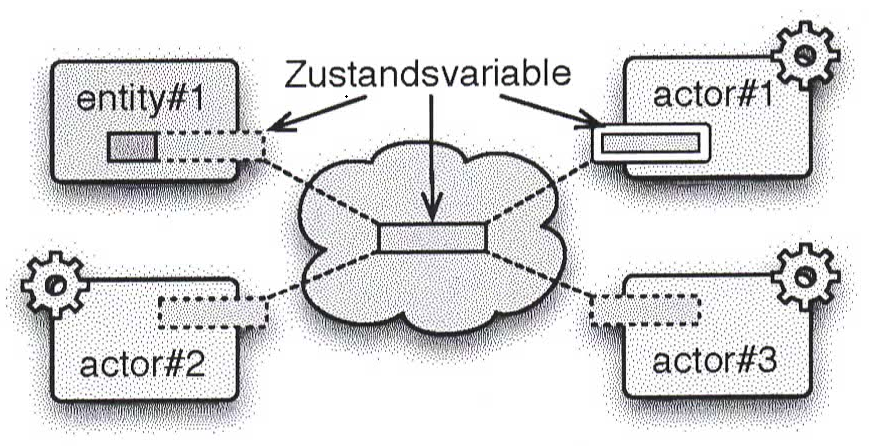
\includegraphics[width=80mm]{bilder/siris_actors.png}
\caption{Referenzierung in SIRIS \autocite{WorldInterface}}
\label{fig:sirisactors}
\end{figure}

Die Architektur von SIRIS basiert auf dem \textit{Actor Pattern}. Actors sind im Gegensatz zu Threads eine high-level Abstraktion von isoliert laufenden, nebenläufigen Prozessen. Jeder Actor kann über Nachrichten mit anderen, ihm bekannten Actors kommunizieren, hat aber keinerlei Einfluss darauf wie, wann und ob die angesprochenen Actors auf die Nachrichten reagieren. Actors sind sehr sicher, da sie keinen gemeinsamen Status haben. Dies vereinfacht den Umgang mit nebenläufigen Prozessen deutlich (für eine sehr gute Einführung siehe \autocite{ActorsInScala}).

In SIRIS gibt es auch ein Event Handling-Modell über das Actors, die sich für Änderungen an einer Zustandsvariable interessieren, benachrichtigt werden sobald sich diese verändert.
\lstset{language=Scala}
\begin{lstlisting}[caption={Registrieren einer Callbackfunktion zur Änderungsüberwachung einer Zustandsvariablen}, label={lst:siriscallback}]
handleEntity('myEntity)(entity => entity match {
  case Some(e) => {
    e.get(Transformation) match {
      case Some(sVar) => observe(sVar, (matrix: Mat4x4) => {
        // Do something with the matrix
      })
      case None => {
        // The entity 'myEntity does not reference a status variable (sVar) of type Transformation.
      }
    }
  case None => {
    // Entity with the name 'myEntity was not found
  }
})
\end{lstlisting}
Listing \ref{lst:siriscallback} mag gerade für Scala-Unerfahrene auf den ersten Blick etwas überfordern. Im Kapitel \ref{chap:umsetzung} wird erläutert was sich genau dahinter verbirgt. Auf die Methode \texttt{handleEntity} wird etwas weiter unten noch kurz eingegangen.

SIRIS verfügt über eine eingebaute Knowledge Representation Layer (Wissensrepräsentationsebene). Entitäten und Zustandsvariablen werden auf Anwendungsebene mit Hilfe der Web Ontology Language (kurz OWL, siehe \autocite{OWL}) beschrieben. Dies deshalb, da die funktionalen Komponenten des Softwaresystems intern häufig eine andere Repräsentation, beispielsweise einer Entität, benötigen und in anderer Weise auf Attribute zugreifen müssen als andere Komponenten. Die Beschreibung liefert einen global gültigen Datentyp und die funktionalen Komponenten erhalten einen für sie konvertierten, lokalen Datentyp mit dem sie arbeiten können. Hierdurch können die Komponenten autonom arbeiten und sind nicht von den lokalen Datentypen in anderen Komponenten abhängig \autocite[44]{EnhancedDecoupling}. Entitäten können hierbei aus verschiedenen Aspekten bestehen, wie beispielsweise einem 3D-Mesh und einer Hüllgeometrie\footnote{Wird beispielsweise von der Physik benötigt, um festzustellen ob ein Objekt mit einem anderen kollidiert ist}. Für das Erstellen von Zustandsvariablen und Entitäten gibt es eine Methode namens \texttt{realize}. In Listing \ref{lst:sirisfassrealisierung} ist ein Beispiel für das Erstellen einer 3D Geometrie-Entität (konkret ein Fass) beschrieben. Der dort dargestellte Code gehört zum Barrelstack-Benchmark von SIRIS und wurde für bessere Lesbarkeit etwas angepasst. So werden \texttt{scale} und \texttt{transform} in Wirklichkeit natürlich mit konkreten Werten initialisiert.
\lstset{language=Scala}
\begin{lstlisting}[caption={Erstellen einer Entität über eine Entitätsbeschreibung}, label={lst:sirisfassrealisierung}]
realize(
  EntityDescription(
    ShapeFromFile(
      file = "assets/vis/barrel/barrel3.dae",
      scale = ConstMat4(...),
      transformation = ReadFromElseWhere
    ),
    PhysCylinder(
      transform = ConstMat4(...),
      radius = 3.0,
      height = 5.0,
      align = Axis.Z,
      mass = 10.0
    )
  ),
  (e : Entity) => println( "Created barrel")
)
\end{lstlisting}
Die \texttt{EntityDescription} enthält zwei Aspekte: ein 3D-Mesh, welches aus einer COLLADA-Datei gelesen wird \texttt{barrel3.dae}, und eine Hüllgeometrie \texttt{PhysCylinder}. Zudem wird eine Callback-Funktion bereitgestellt die aufgerufen wird, sobald die Entität erstellt wurde. In obigem Fall wird dann lediglich "`Created barrel"' auf der Konsole ausgegeben.

Die Registrierung von Entitäten, neuen Actors und Zustandsvariablen geschieht ebenfalls über einen Actor. Sie werden über Symbole, ein Konstrukt aus der Sprache Scala, registriert. Hierbei kann eine Komponente auch über mehrere Symbole registriert werden. Intern werden jedoch Universally Unique Identifiers (kurz UUIDs) verwendet. Diese ermöglichen die eindeutige Identifikation einer registrierten Komponente \autocite[51]{WorldInterface}.

Für jede registrierbare Komponente, sei es eine Zustandsvariable, ein Actor oder eine Entität, gibt es im World Interface eigene Methoden. Listing \ref{lst:sirisentityhandling} zeigt beispielsweise die Methoden für den Umgang mit Entitäten.
\lstset{language=Scala}
\begin{lstlisting}[caption={Methoden zum Registrieren, handlen und deregistrieren von Entitäten}, label={lst:sirisentityhandling}]
registerEntity(name: Symbol, e: Entity) {
  // Register an entity with the given name
}

unregisterEntity(e: Entity) {
  // Unregister a given entity
}

handleEntity(name: Symbol)(handler: Option[Entity] => Any ) {
  // Handle an entity (if exists) with the given name and the given handler function (callback function)
}
\end{lstlisting}
Durch diese Konzentration auf den Zustand von Objekten werden zwei für die Softwarequalität wichtige Aspekte erreicht \autocite[305]{GuruMeditation}:
\begin{itemize}
    \item \textbf{Starke Kohäsion}\\
Kohäsion beschreibt wie gut die in einem Softwaresystem enthaltenen funktionalen Komponenten ihre jeweiligen Aufgaben abbilden. Starke Kohäsion meint hierbei dass jede Komponente nur die von ihr zu leistende Aufgabe erledigt. Ähnlich ist das Unix-Prinzip, ausgedrückt von Doug McIlroy, einem der Begründer der Unix-Philosophie: \begin{quote}"`This is the Unix philosophy: Write programs that do one thing and do it well.[\ldots]"'\footnote{zitiert nach \url{http://www.faqs.org/docs/artu/ch01s06.html} (besucht am 19. August 2012)}\end{quote}
    \item \textbf{Niedrige Kopplung}\\Kopplung beschreibt wie stark funktionale Komponenten in einem Softwaresystem voneinander abhängen. Niedrige Kopplung meint hierbei dass einzelne Komponenten ihre Aufgaben völlig autark und isoliert erledigen können und bestenfalls nichts von der Existenz anderer Komponenten wissen (müssen).
\end{itemize}
SIRIS bildet daher eine moderne, sehr gut erweiterbare Plattform in der sich Komponenten leicht austauschen oder entfernen lassen, ohne dabei andere Komponenten oder gar das zugrunde liegende System verändern zu müssen. Dies erhöht die Wartbarkeit und verringert sowohl die Komplexität selbst geschriebener Anwendungen und verbessert die Lernkurve für neue Entwickler die später in ein Projekt einsteigen und das System (oder zumindest den Teil des Systems an dem sie mitarbeiten werden) erst kennenlernen müssen.
\chapter{Konzeption}
\label{chap:konzeption}
Das im Rahmen dieser Arbeit entwickelte verteilte Echtzeit-3D-Renderingsystem hat den Namen \textit{Osiris}. Der Name bedeutet \textit{Online SIRIS}, da der WebGL-Renderer auf der einen Seite ohne das SIRIS-Backend nicht wie erwartet funktionieren würde und er zudem einige der Möglichkeiten von SIRIS online über den Browser verfügbar macht.
\begin{figure}
\centering
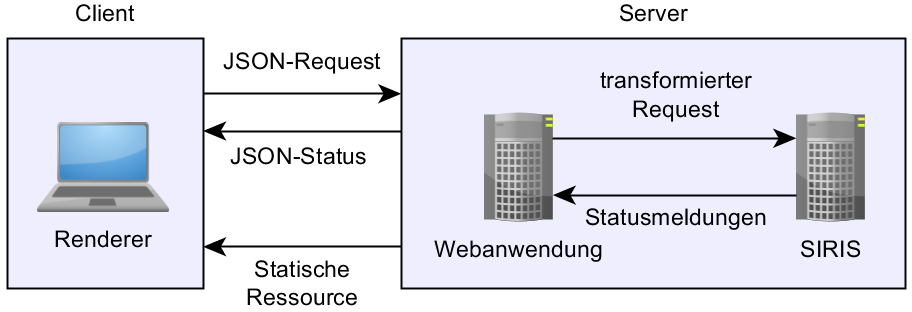
\includegraphics[width=\textwidth]{bilder/structure.png}
\caption{Prinzipielle Sytemstruktur}
\label{fig:structure}
\end{figure}
Osiris besteht aus einem WebGL-Renderer und einem Webserver, der statische Ressourcen bereit stellt und die Kommunikation über eine WebSocketverbindung mit dem SIRIS-Backend steuert. Auf dem Webserver wird auch SIRIS inklusive der angebundenen Physikengine ausgeführt. Dieses Setup überlässt dem Client lediglich das Rendern der 3D-Szene, die rechenintensive Physiksimulation findet auf dem Server statt.

Der WebGL-Renderer sowie die Anwendung auf dem Webserver und die Anbindung an SIRIS wurden eigenständig neu implementiert. SIRIS ist auf dem Stand vom 6. Juni 2012, der Quelltext wurde bis auf das Abschalten des leistungszehrenden Benchmarkings nicht verändert.

In der Webanwendung sind mehrere Controller registriert die auf Anfragen reagieren und dem Client bestimmte Informationen bereitstellen. So gibt es jeweils einen Controller für die WebSocket-Kommunikation, Szenen und Shaderprogramme. Dies macht die Organisation der betreffenden Daten auf dem Server für den Client völlig transparent und verringert die Kopplung der funktionalen Komponenten im System. Um den Fokus auf der Anbindung des Renderers an SIRIS zu erhalten und den Komplexitätsgrad der Anwendung nicht zu weit zu steigern wurde auf die Unterstützung mehrerer Anwender verzichtet, da das Play! Framework statuslos ist und für das Vermeiden der Vermischung von Nachrichten eine recht komplexe Verwaltung der unterschiedlichen Anwender hätte implementiert werden müssen. Dies wäre im kurzen Zeitrahmen für diese Arbeit kaum möglich gewesen.

Der Renderer wird mitsamt der HTML-Seite und der für den Stil verantwortlichen CSS-Datei beim Verbinden mit dem Server an den Browser übertragen. Vor der Auslieferung fügt die Webanwendung Informationen über die verfügbaren Szenen und Shaderprogramme in die Webseite ein. Der Benutzer kann nun die darzustellende Szene und das dafür zu benutzende Shaderprogramm wählen woraufhin beides über den Renderer vom Webserver angefordert wird. Dies ermöglicht eine sehr flexible Bereitstellung neuer Szenen und Shaderprogramme.

Im gegenwärtigen Zustand unterstützt der Renderer Beleuchtung mit verschiedenen Lichtquellen und die Texturierung der dargestellten Objekte mit verschiedenen Texture Map-Typen. Über eine Websocketverbindung kommuniziert der Renderer über fest vordefinierte, in JSON enkodierte Nachrichten mit dem Server. Dieser sendet ebenfalls fest vorgegebene JSON-Nachrichten an den Client. JSON ist die Abkürzung für die \textit{JavaScript Object Notation}. Mit dieser lassen sich komplexe, hierarchische Strukturen in Reintextform beschreiben. Tatsächlich ist jede JSON-Nachricht ein valides JavaScript-Objekt. Diese Festlegung etabliert auf beiden Seiten wohldefinierte Kommunikations-APIs, abstrahiert die auf der jeweiligen Seite ablaufenden Prozesse und macht den Unterschied der verwendeten Programmiersprachen völlig transparent. So könnte man den Renderer auch gegen eine völlig andere funktionale Komponente austauschen, solange diese über die gleichen Nachrichten mit dem Server kommuniziert wie der Renderer. Ein kleinerer Nachteil ist, dass JSON nicht die Kompaktheit von binären Datentypen erreicht.

Die Szene wird ebenfalls mittels JSON beschrieben und enthält alle notwendigen Informationen zu ihrer Darstellung und Interaktion und bildet so einen einfachen Szenegraphen ab. Der Wurzelknoten enthält mehrere Gruppenknoten, denen jeweils bestimmte Knotentypen, wie Kameradaten, Informationen über die in der Szene dargestellten 3D-Objekte, Informationen zur Beleuchtung und die zur Manipulation bestimmter Objekte verwendbaren Tasten zugeordnet sind (siehe Abbildung \ref{fig:szenestruktur} und Listing \ref{lst:scenejson}). Durch die Notation in JSON lassen sich so beliebige Szenen sehr flexibel beschreiben wobei der im Rahmen dieser Arbeit entwickelte Renderer auf die Existenz einiger Knoten angewiesen ist.
\lstset{language=JavaScript}
\begin{lstlisting}[caption={JSON-Struktur einer möglichen Szene}, label={lst:scenejson}]
{
  "type": "scene",
  "rootNode": {
    "id": "root",
    "type": "group",
    "children": [
      {
        "id": "options",
        "type": "group",
        "children": [
          {
            "id": "cam",
            "type": "camera",
            "position": {
              ...
            },
              ...
          },
            ...
      },
      {
        "id": "lights",
        "type": "group",
        "children": [
          ...
        ]
      },
      {
        "id": "models",
        "type": "group",
        "children": [
          ...
        ]
      }
    ]
  }
}
\end{lstlisting}
\begin{figure}
\centering
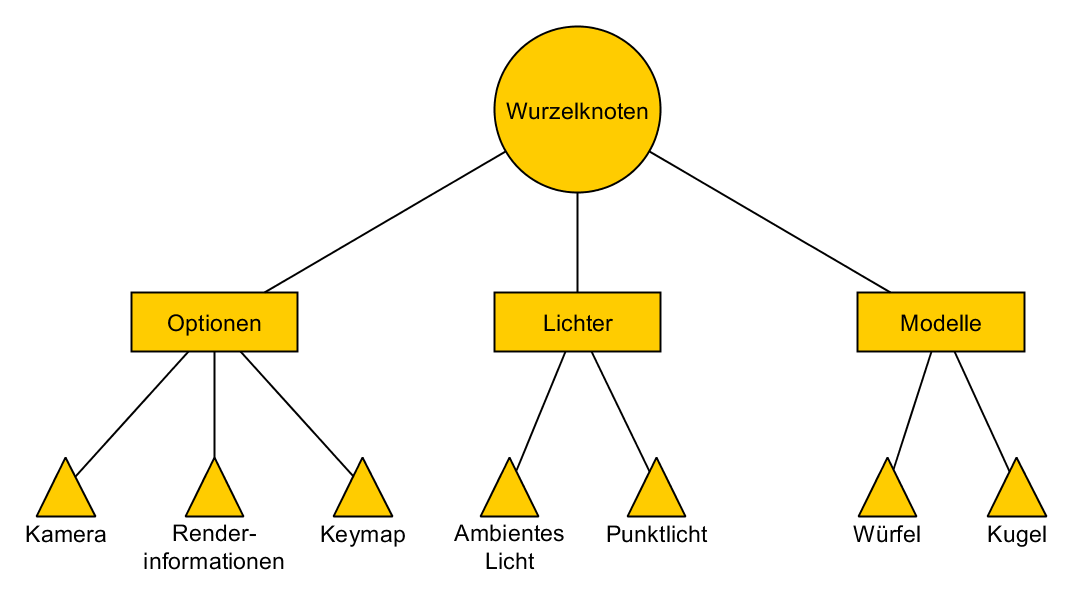
\includegraphics[height=70mm]{bilder/scenestructure.png}
\caption{Beispielstruktur einer Szene}
\label{fig:szenestruktur}
\end{figure}
Auf dem Webserver findet auch die Transformation der JSON-Nachrichten vom Client in ein für SIRIS verständliches Format und umgekehrt von SIRIS an den Client statt. Da sowohl der Renderer als auch die in SIRIS enthaltene Physikengine für jedes Objekt wissen müssen wo es sich wann mit welcher Ausrichtung in der dargestellten Szene befindet, verfügt jeder Objektknoten über eine eigene Transformationsmatrix. Sowohl SIRIS als auch WebGL bilden alle Transformationen in einem Rechtshändigen Koordinatensystem mit den folgenden Vereinbarungen ab:
\begin{itemize}
    \item Die drei Achsen (\textit{x}, \textit{y} und \textit{z}) stehen im rechten Winkel aufeinander.
    \item Die \textit{x}-Achse zeigt nach Osten.
    \item Die \textit{y}-Achse zeigt nach oben in Richtung eines imaginären Himmels.
    \item Die \textit{z}-Achse zeigt nach vorn in Richtung des Betrachters.
\end{itemize}
\begin{figure}
\centering
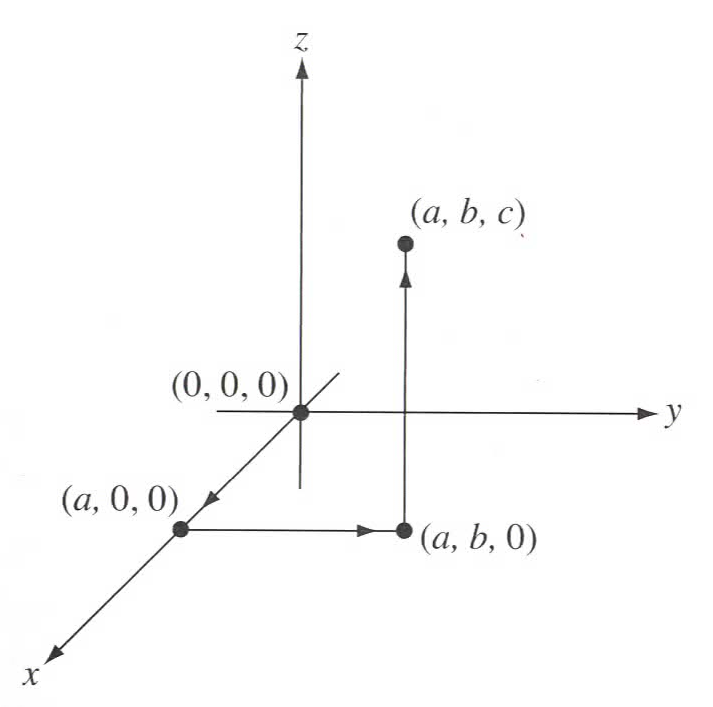
\includegraphics[height=60mm]{bilder/righthandcoordsystem.png}
\caption{Das Rechtshändige Koordinatensystem von JBullet und WebGL}
\label{fig:coordsystem}
\end{figure}
\chapter{Umsetzung}
\label{chap:umsetzung}

\section{Vorbemerkungen zum Renderer}
\label{sec:renderer}
Der Renderer wurde in JavaScript geschrieben da dies die einzige Programmiersprache ist, die clientseitig von jedem modernen Browser ohne manuellen Kompilierunsgprozess, Plugins oder ähnlichem ausgeführt werden kann. Da JavaScript einige Eigenheiten besitzt und für das Schreiben des Renderers eine bestimmte Designphilosophie und Bibliotheken verwendet wurde, werden diese zum besseren Verständnis des Codes im Folgenden erläutert.

\subsection{JavaScript}
JavaScript ist eine sehr ausdrucksstarke Sprache, die es dem Programmierer ermöglicht mit wenigen Codezeilen sehr elegante und schlanke Anwendungen zu schreiben. Allerdings hat JavaScript bei vielen bis heute auch einen negativen Ruf. Nachfolgend einige Gründe hierfür:
\begin{itemize}
    \item Einige Teile der Sprache sind für Programmierer die bisher mit klassischen Programmiersprachen (C/C++, Java, etc.) gearbeitet haben schwer verständlich und unintuitiv, wie Prototypische Vererbung, das komplette Fehlen von Klassen, die im Vergleich sehr geringe Anzahl an Objekten für bestimmte Aufgaben ("`Klassenbibliothek"') oder die Verwendung mancher Sprachkonstrukte, wie dem \textit{Date}-Objekt.
    \item Schon kleine Fehler, wie ein vergessenes Semikolon, ein vergessener \textit{new} Operator oder ein vergessenes \textit{var} bei der Deklaration von Variablen, können zu unvorhersehbarem Programmverhalten und schwer auffindbaren Fehlern führen. Anders als klassische Sprachen werden die drei genannten Aspekte vom Interpreter nicht als Fehler gehandhabt, sondern als gültiger Code verarbeitet da sie bereits beim Sprachdesign so eingebaut wurden.
    \item JavaScript kennt das Prinzip von Namespaces oder Packages nicht, sondern arbeitet mit globalen Variablen. Dies kann in Verbindung mit fremden JavaScript-Code zu ernsthaften Konflikten führen und macht die Entwicklung von komplexeren und größeren Anwendungen schwerer als in anderen Sprachen.
\end{itemize}
Trotz des schlechten Rufs hat JavaScript aber auch einige sehr gute Seiten, welche die Sprache wirklich attraktiv machen und die man in manchen etablierten Sprachen schnell vermisst. Nachfolgend eine (sehr kleine) Auswahl:
\begin{itemize}
    \item Funktionen sind Objekte erster Klasse. Das heißt, sie können eigenständig existieren, über Variablen referenziert und als Rückgabetypen von anderen und als Parameter in andere Funktionen zurückge-/übergeben werden. Funktionen können auch auch andere Funktionen als Attribute haben.
    \item Funktionen können als sogenannte Lambdafunktionen anonym verwendet werden. Dadurch müssen sie vor Gebrauch nicht erst benannt oder einer Variablen zugewiesen werden.
    \item Objekte können zur Laufzeit beliebig erstellt und um neue Attribute und Funktionen erweitert werden.
\end{itemize}
Der JavaScript-Guru Douglas Crockford hat ein Buch über die "`Good Parts"' (guten Seiten) der Sprache geschrieben \autocite{JsGoodParts}, in dem er auch die "`Bad Parts"' (schlechten Seiten) aufzeigt und Strategien erläutert, wie man diese möglichst elegant umgehen kann. Dieses Buch sei an dieser Stelle jedem empfohlen der sich etwas tiefer mit der Sprache beschäftigen oder einfach nur komplexere, wartbare Anwendungen damit entwickeln möchte.

ECMAScript\footnote{\url{http://www.ecmascript.org/} (besucht am \today)} ist der offizielle Name des Standards auf dem JavaScript aufbaut, und beide Begriffe werden häufig synonym verwendet. Jedoch ist JavaScript "`nur"' ein ECMAScript-Dialekt. Weitere Dialekte sind beispielsweise ActionScript\footnote{\url{http://www.adobe.com/devnet/actionscript.html} (besucht am \today)} von Adobe (bekannt für die Flashprogrammierung). Die Entwicklung von JavaScript schreitet kontinuierlich voran und wird derzeit vor allem durch HTML5 beschleunigt. JavaScript ist eine interpretierte Sprache, für die von jedem Browserhersteller eine Laufzeitumgebung eingebaut werden muss. Dies führt zwar einerseits dazu dass heutige Browser immer schnellere JavaScript-Egines mitliefern, andererseits jedoch sind nicht alle Sprachfeatures (insbesondere die neueren) in jedem Browser verfügbar. Für viele Webentwickler ist es ein Teil der täglichen Arbeit Code auch mit älteren Browsern kompatibel zu machen.

Mit den Versionen ECMAScript 5 und 6 werden viele Verbesserungen in die Sprache Einzug halten, von denen die aktuellen Versionen moderner Browser bereits einige unterstützen, wie den \textit{Strict Mode}. In diesem Modus wird die Verwendung einiger besonders fehlerträchtiger Sprachkonstrukte, wie die \textit{with}- und \textit{eval}-Statements als Fehler gewertet und der Code kann nicht ausgeführt werden. Dieser Modus hilft gerade durch seine Einschränkungen jedoch validen und wartbaren Code zu schreiben und meiner Einschätzung nach sollten neue Pojekte immer mit aktiviertem Strict Mode geschrieben werden. Hierbei wird empfohlen ihn innerhalb der hierarchisch höchsten Funktion zu deklarieren, um Konflikte mit nicht Strict Mode-fähigem Fremdcode zu vermeiden. Der Strict Mode wird über den einfachen String \textit{"`use strict"'} aktiviert. Hierdurch können auch ältere Browser, die ihn nicht unterstützen, den Code ausführen da das Statement nur ein einfacher String ist. In Osiris ist jedes Modul im Strict Mode geschrieben.
\lstset{language=JavaScript}
\begin{lstlisting}[caption={Aktivierung des \textit{Strict Mode}}]
function doSomething() {
"use strict"

// rest of the code
}
\end{lstlisting}
Um einige der negativen Seiten zu beheben, oder dem Programmierer zumindest Möglichkeiten an die Hand zu geben sie zu vermeiden, sind vor allem im Laufe der letzten Jahre eine große Menge verschiedener JavaScript-Frameworks und Bibliotheken veröffentlicht worden. Darunter finden sich sowohl umfassende Alleskönner wie das Dojo Toolkit\footnote{\url{http://dojotoolkit.org/} (besucht am \today)} als auch sehr raffinierte Werkzeuge für spezielle Aufgaben, wie die AsyncJs-Bibliothek\footnote{\url{https://github.com/caolan/async} (besucht am \today)}.

Für die Umsetzung des WebGL-Renderers wurden ebenfalls einige Bibliotheken verwendet die teilweise auch die Architektur der Anwendung mitbestimmt haben. Um den Code zu verstehen ist es daher notwendig diese kurz vorzustellen.

\subsection{RequireJs}
RequireJs versucht das aus etablierten Sprachen nicht mehr wegzudenkende Konstrukt der Namensräume in JavaScript nachzubilden. Hierbei werden funktionale Komponenten in sogenannte "`Module"' verpackt, die von anderen Modulen abhängig sein können (ähnlich dem \textit{import}-Statement in Java) und anderen Modulen eine öffentliche Schnittstelle für den Umgang mit dem Modul bereitstellen. Dies verbessert die Codeorganisation enorm. Zudem übernimmt RequireJs das asynchrone Laden von benötigten Modulen, was zu einer Reduzierung des benötigten Codes führen kann und das Laden beim Seitenaufruf beschleunigt. Die Entwickler von RequireJs haben hierfür den Begriff \textit{Asynchronous Module Definition} (kurz AMD) eingeführt. Mittlerweile sind auch andere JavaScript-Bibliotheken nach diesem Muster aufgebaut oder bieten das Laden von nach AMD geschriebenen Modulen an.
\lstset{language=JavaScript}
\begin{lstlisting}[caption={Aufbau eines Moduls nach AMD in Osiris}, label={lst:amd}]
define(["zepto"], function($) {
  "use strict";

  function _visit(node, executor) {
    // private method. Only accessible inside this module
  }

  return {
    execute: function(traversableScene, executor) {
      // public method. Is part of the module's API
    }
  };
});
\end{lstlisting}
Der Code in Listing \ref{lst:amd} definiert ein namensloses (empfohlen) Modul mit den Abhängigkeiten auf das Modul \textit{zepto}. Abhängigkeiten werden immer als Strings in einem Array am Anfang der \texttt{define}-Funktion angegeben. Um auf die Module zugreifen zu können werden Referenzen auf sie in der folgenden anonymen Funktion an das Modul übergeben. Die Referenzen können auch anders heißen als das Modul selbst. Im vorliegenden Code wird das Modul \textit{zepto} über den Namen \textit{\$} referenziert. Dadurch ist es möglich auf öffentliche Egenschaften und Methoden dieses Moduls zuzugreifen. Das \texttt{return}-Statement gibt ein Objekt mit der öffentlichen API des Moduls zurück, über welche andere Module mit diesem Modul interagieren können (in diesem Falle nur die \texttt{execute}-Methode).

Statt in der HTML-Seite nun jede JavaScript-Datei einzeln zu referenzieren, legt man lediglich einen \texttt{<script>}-Tag an, in welchem RequireJs geladen und die Hauptausführungsdatei (Main) der Anwendung referenziert wird.
\lstset{language=HTML}
\begin{lstlisting}[caption={Referenzierung einer RequireJs-Anwendung in einer Play! Framework Template}, label={lst:requireJsInPlayreferenzieren}]
<script data-main="assets/javascripts/main" src="@routes.Assets.at("javascripts/lib/require.js")"></script>
\end{lstlisting}
Bei dem Code in Listing \ref{lst:requireJsInPlayreferenzieren} ist zu beachten, dass dies die Einbettung in der View Template des Play! Frameworks darstellt. Mehr dazu folgt im Kapitel \ref{chap:konzeption} \textit{Konzeption}.

Die über das \texttt{data-main} Attribut referenzierte Datei enthält nun die Konfiguration der verfügbaren Module.
\lstset{language=JavaScript}
\begin{lstlisting}[caption={Konfiguration der verfügbaren Module}, label={lst:konfigurationModule}]
require.config({
  // Non AMD scripts that add themselves to the global object
  shim: {
    "async": {
      exports: "async"
    },
    "zepto": {
      exports: "$"
    }
  },

  paths: {
    // app
    Osiris: "Osiris",

    // libraries
    zepto: "lib/zepto",
    async: "lib/async",

    ...

    // infrastructure
    SendMessage: "infrastructure/SendMessageToServer",

    ...
  }
});
\end{lstlisting}
Hierbei werden die Module benannt und der relative Pfad angegeben, unter dem die Moduldatei liegt (ohne die Endung \texttt{.js}). Bibliotheken, die nicht dem AMD-Schema folgen können über das \texttt{shim}-Objekt dennoch als solche behandelt werden.

RequireJs bietet noch einige Funktionen mehr, beispielsweise das Optimieren und Zusammenführen aller Module in einer Datei für das schnellere Laden, von denen ich allerdings im Rahmen dieser Arbeit keinen Gebrauch gemacht habe. Ohne RequireJs wäre es jedoch sehr viel schwieriger geworden separierten und gut wartbaren Code zu schreiben.

\subsection{AsyncJs}
In JavaScript gab es lange keine Threads (außer dem eigenen Anwendungsthread). Lang laufende Skripte blockierten die Anwendung und konnten dazu führen, dass im Browser ein Timeout erzeugt wurde und der Anwender eine Nachricht erhielt, dass das Skript möglichweise nicht richtig funktioniert. Im Rahmen von HTML5 wird versucht diesen Missstand mit Hilfe eines neuen, noch in der Entwicklung befindlichen, Standards zu beheben, den \textit{Web Workers}. Diese bieten die Möglichkeit komplexere Aufgaben, wie das Herunterladen großer Dateien oder komplexe Berechnungen, in separaten Threads auszuführen.

Als Alternative zu den Web Workers hat sich das asynchrone Callback-Pattern etabliert. Da Funktionen in JavaScript Objekte erster Klasse sind, können sie auch an andere Funktionen als Parameter übergeben und innerhalb dieser aufgerufen werden. Hierdurch blockiert der Aufruf einer Funktion nicht die komplette Anwendung. Diese kann mit anderen Dingen fortfahren und kann über das registrierte Callback auf das Ergebnis der angestoßenen Funktion reagieren, obwohl alles nur in einem Thread abläuft. Dies nennt man \textit{reaktive} oder \textit{eventgetriebene} Programmierung.
\begin{figure}
\centering
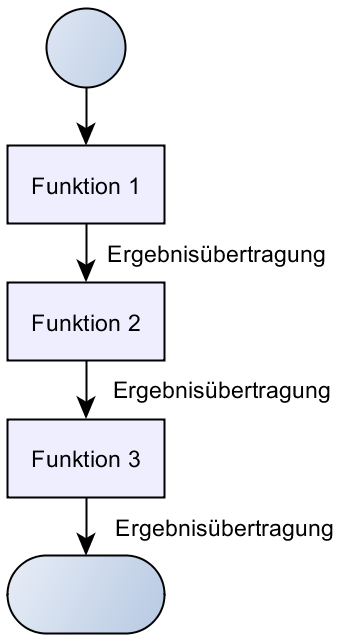
\includegraphics[height=80mm]{bilder/asyncwaterfall.png}
\caption{Beispielablauf der Funktion \texttt{waterfall} aus AsyncJs}
\label{fig:asyncwaterfall}
\end{figure}
Bei der Implementierung des Renderers fiel die Entscheidung aus pragmatischen Gründen für das Callback-Pattern, da für Web Worker erheblich mehr Aufwand betrieben werden muss und die vom Renderer parallel ausgeführten Tasks nicht so komplex sind, dass sie die komplette Anwendung einfrieren lassen können. Web Worker werden in einer eigenen, sehr abgeschotteten Umgebung ausgeführt in der nicht alle Möglichkeiten von JavaScript zur Verfügung stehen. Zudem ist die Integration mit RequireJs noch nicht auf unkomplizierte Weise gelöst.
\lstset{language=JavaScript}
\begin{lstlisting}[caption={Beispiel für eine Methode mit einem Callback}, label={lst:funktionmitcallback}]
function downloadFileFromUrl(url, callback) {
  var file;

  // download the file's contents into the file variable

  callback(file);
}
\end{lstlisting}
\lstset{language=JavaScript}
\begin{lstlisting}[caption={Beispiel für ein mögliches Callback}, label={lst:callbackbeispiel}]
var callback = function(file) {
  window.alert(file);
}
\end{lstlisting}
In Listing \ref{lst:funktionmitcallback} wird anhand einer einfachen Funktion gezeigt, wie am Ende einer Funktion das Ergebnis statt per \texttt{return} an den Aufrufer zurück, es an das registrierte Callback übergeben und dieses aufgerufen wird. Das Callback könnte dabei so aussehen wie in Listing \ref{lst:callbackbeispiel}, welches den Inhalt der Datei über eine Benachrichtigung auf dem Bildschirm darstellen würde.

Callbacks sind eine sehr gut Möglichkeit um mehrere Aufgaben parallel laufen zu lassen. Jedoch weiß man nie wann und ob ein Callback ausgeführt wird. Wenn die weitere Ausführung von Programmcode beispielsweise von den Ergebnissen mehrerer paralleler Aufgaben abhängig ist, muss vom Programmierer garantiert werden dass der nächste Schritt erst gestartet wird nachdem alle relevanten Callbacks ausgeführt wurden und ihre Ergebnisse geliefert haben.

Die AsyncJs-Bibliothek bietet hier Abhilfe. Über die in ihr enthaltenen Funktionen lassen sich auch komplexe asynchrone Abläufe sehr gut steuern. Zudem werden auch Funktionen angeboten mit denen Collections, wie Arrays und Objekte parallel verarbeitet werden können.
\lstset{language=JavaScript}
\begin{lstlisting}[caption={Beispiel für einen Aufruf von AsyncJs}, label={lst:asyncjsbeispiel}]
Async.waterfall([
  function(callback) {
    DownloadSceneFromServer.execute(sceneInformation, callback);
  },
  function(downloadedScene, callback) {
    PrepareSceneForRendering.execute(downloadedScene, glContext, callback);
  }
], _onComplete);
\end{lstlisting}
Wie Listing \ref{lst:asyncjsbeispiel} exemplarisch zeigt wird in der Regel ein Hauptcallback (\texttt{\_onComplete}) angegeben welches ausgeführt wird, sobald alle Funktionen ihr jeweiliges lokales Funktionscallback aufgerufen haben. Diesem Hauptcallback können aufgetretene Fehler oder erreichte Ergebnisse mitgegeben werden. Ein mögliches Hauptcallback ist in Listing \ref{lst:asyncjscallbackbeispiel} zu sehen. Die Abbildungen \ref{fig:asyncwaterfall}, \ref{fig:asyncparallel} und \ref{fig:asyncauto} zeigen den Ablauf von dreien der in der Bibliothek enthaltenen Funktionen.
\lstset{language=JavaScript}
\begin{lstlisting}[caption={Beispiel eines Hauptcallback für Listing \ref{lst:asyncjsbeispiel}}, label={lst:asyncjscallbackbeispiel}]
function _onComplete(error, preparedScene) {
  if (error) {
    throw error;
  }
  RenderScene.execute(preparedScene);
}
\end{lstlisting}
\begin{figure}
\centering
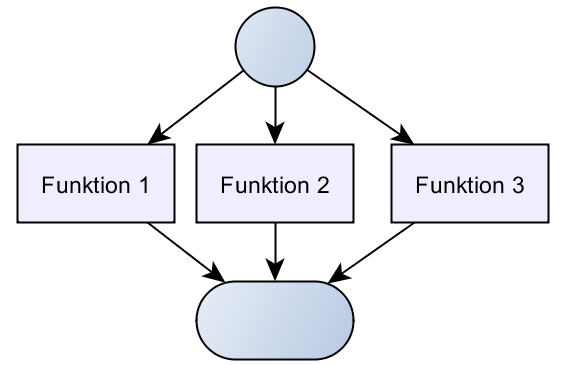
\includegraphics[width=70mm]{bilder/asyncparallel.png}
\caption{Beispielablauf der Funktion \texttt{parallel} aus AsyncJs}
\label{fig:asyncparallel}
\end{figure}
Für Osiris sind drei der AsyncJs-Funktionen von besonderer Bedeutung, denn sie bestimmten das Ablaufverhalten einiger Module maßgeblich:
\begin{enumerate}
    \item \textbf{async.parallel}\\
Führt gegebene Funktionen gleichzeitig (parallel) aus. Die Ergebnisse oder Fehler werden für jede beendete Funktion an das Hauptcallback geliefert. Dieses hat nun Zugriff auf alle Ergebnisse.
    \item \textbf{async.waterfall}\\
Führt gegebene Funktionen nacheinander aus und übergibt das Ergebnis der Vorgängerfunktion an die nachfolgende. Das Ergebnis der letzten Funktion wird an das Hauptcallback geliefert.
    \item \textbf{async.auto}\\
Erstellt einen Abhängigkeitsgraphen der registrierten Funktionen und führt sie so aus, dass Funktionen mit gleichen Abhängigkeiten parallel ausgeführt werden sobald die Abhängigkeiten erfüllt sind.
\end{enumerate}
Durch die Verwendung von AsyncJs war es möglich viele Vorgänge, wie das Herunterladen und Vorbereiten von Szene und Shaderprogramm, gleichzeitig ablaufen zu lassen und so die Verarbeitung zu beschleunigen. Zudem lassen sich mögliche Abhängigkeiten beispielsweise über die \texttt{async.auto}-Funktion sehr leicht beschreiben und die Verwaltung der verschiedenen Callbacks für jedes Modul über das Hauptcallback stark erleichtern. Denn eine besondere Schwierigkeit bei vielen Callbacks ist nicht den Überblick zu verlieren und so schwer auffindbare Fehler in den Programmcode einzubauen.
\begin{figure}
\centering
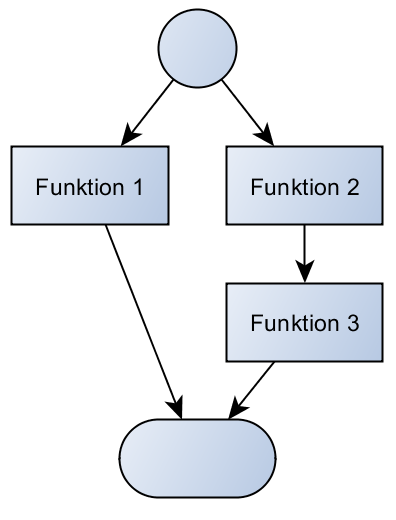
\includegraphics[height=70mm]{bilder/asyncauto.png}
\caption{Beispielablauf der Funktion \texttt{auto} aus AsyncJs}
\label{fig:asyncauto}
\end{figure}
\subsection{Weitere Bibliotheken}
Die restlichen Bibliotheken haben die Struktur des Renderer-Codes nicht maßgeblich beeinflusst, weshalb ihre Aufgaben nur kurz erwähnt werden.
\begin{itemize}
    \item \textbf{glMatrix}\\
GlMatrix ist eine speziell für WebGL entwickelte Matrizen- und Vektorenbibliothek. Mit ihr lassen sich komfortabel und sehr schnell allgemeine Berechnungen durchführen und sie enthält einige Funktionen die die Arbeit mit WebGL vereinfachen, wie \texttt{perspective} und \texttt{lookAt}.
    \item \textbf{WebGL Utils}\\
Eine von Google entwickelte Bibliothek die den Umgang mit dem WebGL-Kontext vereinfacht. Sie prüft automatisch ob der verwendete Browser WebGL beherrscht und erstellt eine Fehlerseite mit Informationen, falls nicht.
    \item \textbf{Log}\\
Ein kleiner selbstgeschriebener Wrapper für JavaScript-Logging. Wenn es im Browser kein \texttt{Console}-Objekt und daran bestimmte Methoden gibt, werden die Log-Nachrichten als Benachrichtigungsdialoge ausgegeben.
    \item \textbf{Zepto}\\
Zepto ist eine Bibliothek die hauptsächlich zur DOM\footnote{Document Object Model}-Manipulation gedacht ist und eine ähnliche API wie jQuery anbietet. Dabei ist sie aber deutlich kleiner als ihr Vorbild, da sie keine Unterstützung für alte Browser (z.B.: Firefox < Version 4) oder den Internet Explorer mitbringt.
\end{itemize}

\subsection{Flow Based Programming}
\begin{figure}
\centering
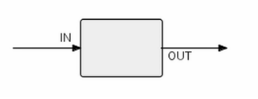
\includegraphics{bilder/fbp_component.png}
\caption{Schaubild einer Elementary Component \autocite{FlowBasedProgramming}}
\label{fig:fbpkomponente}
\end{figure}
In der klassischen Objektorientierung hat man Datenobjekte an denen Methoden (und unter Umständen auch Zustand) angeheftet sind, wie beispielhaft in Listing \ref{lst:ooptextdateibeispiel} zu sehen.
\lstset{language=JavaScript}
\begin{lstlisting}[caption={Beispiel für das objektorientierte Umbrechen einer Textdatei in JavaScript}, label={lst:ooptextdateibeispiel}]
var textFile = new TextFile();
textFile.load("some_text.txt");
textFile.wrapAtLine(80);
var success = textFile.save("wrapped_text.txt");

if (success) {
  window.alert("Text was read, wrapped and saved.");
} else {
  window.alert("Text could not be read, wrapped, and saved.");
}
\end{lstlisting}
Dies wirft einige Probleme auf, da hierbei verschiedene Aspekte zusammengeworfen werden. Das Objekt verletzt das Separation of Concerns-Prinzip, es "`tut"' zu viel: Zuerst greift es lesend auf das Dateisystem zu, liest den Inhalt der referenzierten Textdatei aus, bricht ihn um und speichert den modifizierten Inhalt wieder im Dateisytem. Zudem muss der Programmierer definitiv wissen in welcher Reihenfolge die Methoden des Objekts aufgerufen werden müssen. Im Beispiel ist es noch eine kleine Klasse. In der realen Welt entstehen jedoch oft sehr große Klassen die verschiedenste Aspekte in sich vereinen. Oftmals fällt es auch neuen Teammitgliedern schwer sich in die Architektur bereits bestehender Projekte einzulesen, da beispielsweise ein "`ResourceManager"' nicht auf den ersten Blick verrät welche Aufgaben tatsächlich über ihn abgewickelt werden.

Das Konzept des \textit{Flow Based Programming} (kurz FBP) wurde bereits in den späten 1960er Jahren von John Paul Morrison entwickelt und gewinnt heute durch die immer wichtiger werdende Nebenläufige Pogrammierung und die steigende Komplexität der zu entwickelnden Anwendungen wieder an Gewicht. Es unterscheidet sich in grundlegender Weise von der objektorientierten Herangehensweise, da hierbei nicht Datenstrukturen sondern funktionale Komponenten im Vordergrund stehen. Im FBP werden funktionale Einheiten als Black Box-Komponenten über ihr Verhalten und die eingehenden und ausgehenden Datenflüsse beschrieben. In Abbildung \ref{fig:fbpkomponente} wird eine einzelne Komponente dargestellt. Oftmals verfügen FBP-Komponenten lediglich über einen Ein- sowie Ausgang, können aber beliebig viele davon aufweisen. Jedoch sollte man hierbei strikt im Hinterkopf behalten, dass die Komponente als Ziel nur den zu erfüllenden Aspekt hat. Auf diese Weise sind sie so sehr leicht austausch- und in anderen Kontexten wiederverwendbar. Zudem erlauben sie dem Programmierer sich auf die Algorithmen für das Erledigen einer Aufgabe, sowie die Datenflüsse und die notwendigen Transformationen zu konzentrieren und verletzen die Clean Code-Prinzipien nicht.

Komponenten können auch andere Komponenten enthalten um ihre Aufgabe zu erledigen. Sie exportieren dieselben Schnittstellen wie einfache Komponenten, verbinden diese intern miteinander und dienen dem Programmierer so als Fassade zum komplexeren Vorgang. Diese Art von Komponente wird als \textit{Composite Component}, einfache Komponenten hingegen als \textit{Elementary Component} bezeichnet \autocite{FlowBasedProgramming}.\\
In Abbildung \ref{fig:fbpkomponenten} wird eine mögliche Composite Component dargestellt.
\begin{figure}
\centering
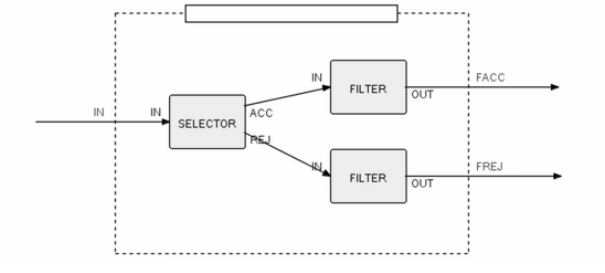
\includegraphics{bilder/fbp_components.png}
\caption{Schaubild einer Composite Component \autocite{FlowBasedProgramming}}
\label{fig:fbpkomponenten}
\end{figure}
Listing \ref{lst:fbptextdateibeispiel} zeigt den gleichen Vorgang wie im objektorientierten Beispiel in Listing \ref{lst:ooptextdateibeispiel} mit Flow Based Components.
\lstset{language=JavaScript}
\begin{lstlisting}[caption={Beispiel für das flussbasierte Umbrechen einer Textdatei in JavaScript}, label={lst:fbptextdateibeispiel}]
function WrapTextFileDemo() {
  var _readText,
    _wrapText,
    _saveText,

    _destPath,
    _wrapAtLine;

  _setup();
  _wire();

  function _setup() {
    _readText = new ReadTextFile();
    _wrapText = new WrapText();
    _saveText = new SaveTextFile();
  }

  function _wire() {
    _readText.onDone = function(readText) {
      _wrapText.execute(readText, _wrapAtLine);
    };

    _wrapText.onDone = function(wrappedText) {
      _saveText.execute(wrappedText, _destPath);
    };

    _saveText.onDone = function(success) {
      if (success) {
        window.alert("Text was read, wrapped and saved.");
      } else {
        window.alert("Text could not be read, wrapped, and saved.");
      }
    };
  }

  this.execute = function(sourceTextFilePath, destinationTextFilePath, wrapAtLine) {
    _wrapAtLine = wrapAtLine;
    _destPath = destinationTextFilePath;

    _readText.execute(sourceTextFilePath);
  };
}

var wrapTextFile = new WrapTextFileDemo();
wrapTextFile.execute("some_text.txt", "wrapped_text.txt", 80);
\end{lstlisting}
Der Code in Listing \ref{lst:fbptextdateibeispiel} zeigt, dass jede Aufgabe von einer spezialisierten Komponente übernommen wird. Diese werden, ähnlich wie in einem Baukastensystem, über ihre Ein- und Ausgänge miteinander verbunden, im Beispiel durch die private Methode \texttt{\_wire} ("`verdrahten"') realisiert. Wenn die erste Komponente \texttt{readText} ausgeführt wird "`fließen"' (daher auch der Name \textit{Flow Based}) die Daten durch die Komponenten hindurch und werden transformiert, bis am Ende das gewünschte Ergebnis erreicht ist. Alle Komponnenten bieten hierbei zum Start die \texttt{execute}-Methode an, der die notwendigen Parameter mitgegeben werden. Dies hat sich als Vereinbarung bewährt.

In obigem Beispiel ist zu sehen, dass sich die FBP-Komponenten in JavaScript mit objektorientierten Möglichkeiten implementieren und mit Callbacks als Ausgänge auch asynchron ausführen lassen. In diesem Fall wurden der Verständlichkeit halber alle Ausgänge \texttt{onDone} genannt. Über diese werden die Ergebnisse der in den einzelnen Komponenten durchgeführten Vorgänge nach außen mitgeteilt. Die Hauptkomponente \texttt{WrapTextFileDemo} ist als Composite Component realisiert und gibt den Erfolgsstatus am Ende direkt im Browser aus.

Für das Verständnis des Codes des Osiris-Renderers sollte diese kurze Einführung ausreichen. John Paul Morrison hat ein Buch über FBP geschrieben, welches das Paradigma sehr detailliert beschreibt \autocite{FlowBasedProgramming}.

\section{Vorbemerkungen zur Webanwendung}
Als Plattform für die Webanwendung und WebSocket-Server wurde das Play! Framework eingesetzt. Ein Framework für die Webanwendung einzusetzen war der schnellste Weg um die benötigte Serverinfrastruktur aufzubauen sowie die Implementierung und Anbindung des Renderers an SIRIS vornehmen zu können. Das Play! Framework bietet hierbei eine, im Gegensatz zu vielen etablierten Java oder Scala Web Frameworks, fast konfigurationsfreie Ausgangsbasis und enthält alle benötigten Konstrukte. Im folgenden Abschnitt werden die für Osiris relevanten Bestandteile kurz erläutert.

\subsection{Play! Framework}
Das Play! Framework ist für die Erstellung von modernen Webanwendungen in Java oder Scala entwickelt worden. Es ist es ein vollständig integriertes Paket in dem alles nötige, wie der Webserver und ORM-Mapper, bereits enthalten ist. Als Webserver wird Jetty (inklusive WebSocket-Protokoll) eingesetzt. Webanwendungen werden mittels des Model View Controller-Architekturmusters realisiert. In Version 2 ist der Quelltext von Java nach Scala portiert worden und die internen Klassen wurden auf das Akka\footnote{\url{http://akka.io/} (besucht am \today)} Actor-Framework umgestellt. Play! ist wie HTTP komplett statuslos, es müssen also alle relevanten Informationen bei jeder Anfrage mitgeschickt werden. Der Vorteil ist jedoch die sehr gute Skalierbarkeit. Da Version 2 noch sehr neu ist, ist die offizielle Dokumentation die Hauptreferenzquelle \autocite{PlayDoku}. Im Frühjahr 2013 werden wohl die ersten Bücher über Play! Version 2 in den Handel kommen\footnote{Der Verlag Manning Publications Co. wird je ein Buch für Java- und Scala-Entwickler herausgeben. \url{http://www.manning.com/hilton/} (besucht am \today)}.

HTTP-Anfragen werden vom Server angenommen und dann gemäß den Regeln in der \textit{routes}-Datei an einen Controller geleitet. Listing \ref{lst:playroutes} zeigt die Regeln für die Controller von Osiris. Hierbei wurde der \textit{Asset-Controller} ausgelassen. Dieser ist Teil des Frameworks und dient zum Herunterladen statischer Ressourcen über direkte Links. Von links nach rechts wird zuerst der akzeptierte HTTP-Anfragetyp deklariert. Dann die relative URL an die der Client anfragt und als letztes der angesprochene Controller und die öffentliche Methode, die ausgeführt werden soll.
\lstset{language=Scala}
\begin{lstlisting}[caption={Regeln für das Weiterleiten von HTTP-Anfragen an Controller}, label={lst:playroutes}]
GET   /         controllers.Application.index
POST  /shaders  controllers.ShaderController.getShaderConfigurationByFilename
POST  /scenes   controllers.SceneController.getSceneByFilename
GET   /socket   controllers.OsirisController.socket
\end{lstlisting}
Das Play! Framework bietet eine sehr leistungsfähige Template Engine. Statt wie in Version 1.x Groovy wird jetzt auch hier Scala verwendet. So können Datentypen vom Controller an die Template übergeben und dort in den HTML-Code eingebaut werden. Listing \ref{lst:playtemplates} zeigt ein Beispiel aus Osiris. Hierbei werden die Informationen zu den verfügbaren Szenen und Shaderprogrammen in ein HTML \textit{select}-Element (Dropdown-Box) integriert, sodass der Anwender später jeweils eins davon auswählen kann.
\lstset{language=HTML}
\begin{lstlisting}[caption={Integrieren der Informationen zu den verfügbaren Szenen und Shadern in ein HTML Select-Element}, label={lst:playtemplates}]
@(sceneInformation: Array[SceneInformation], shaderInformation: Array[ShaderConfiguration])

 ...

  <select id="availableScenes">
    @for(info <- sceneInformation) {
      <option value="@info.file">@info.name</option>
    }
  </select>

    ...

  <select id="availableShaders">
    @for(info <- shaderInformation) {
      <option value="@info.config">@info.name</option>
    }
  </select>
\end{lstlisting}
Für Osiris besonders relevant ist auch die JSON-Behandlung, denn alle ein- und ausgehenden Nachrichten sind so enkodiert. Das Framework bietet eine eigene JSON-Bibliothek an mit welcher es recht einfach ist JSON zu parsen oder zu erzeugen (siehe Listing \ref{lst:playjson}). Es können auch Reader und Writer für benutzerdefinierte Datentypen implementiert werden. Jedoch wurde aufgrund der wenigen benötigten Informationen hierauf verzichtet.
\lstset{language=Scala}
\begin{lstlisting}[caption={Erstellen und parsen eines JSON-Objekts}, label={lst:playjson}]
// Create JSON-Object from primitive values
val shaderInfo = Json.toJson(
  Map(
    "name" -> Json.toJson("Phong"),
    "vertexShader" -> Json.toJson(vertexShaderCode),
    "fragmentShader" -> Json.toJson(fragmentShaderCode),
    "bindables" -> Json.toJson(bindables)
  )
)

// Parse the created object
val name = (shaderInfo \ "name").as[String]
\end{lstlisting}
Eine Websocketverbindung aufzubauen ist sehr einfach. Hierzu werden die Datentypen \textit{Iteratee} und \textit{Enumerator} verwendet, die den Umgang mit Datenströmen abstrahieren. Iteratees werden zum Konsumieren des eingehenden Datenstroms verwendet, Enumeratoren für das Ausgeben der Nachrichten an den Client. Der Code in Listing \ref{lst:playwebsocket} stammt aus der offiziellen Play!-Doku\footnote{\url{http://www.playframework.org/documentation/2.0.3/ScalaWebSockets} (besucht am \today)}. Dort wird folgendes Verhalten gezeigt. Wenn sich ein Benutzer über ein Websocket mit dem Server verbindet, sendet dieser ein "`Hello!"' und schließt die Verbindung. Auf Serverseite wird hiernach zudem ein "`Disconnected"' auf der Konsole ausgegeben.
\lstset{language=Scala}
\begin{lstlisting}[caption={Empfangen und Senden über ein WebSocket in Play!}, label={lst:playwebsocket}]
def index = WebSocket.using[String] { request => 
  // Log events to the console
  val in = Iteratee.foreach[String](println).mapDone { _ =>
    println("Disconnected")
  }
  
  // Send a single 'Hello!' message
  val out = Enumerator("Hello!")
  
  (in, out)
}
\end{lstlisting}

\section{Anwendungsstruktur}
Beim Design von Osiris wurde darauf geachtet eine möglichst klare Struktur für das Projekt zu erreichen. Osiris besteht aus drei Teilprojekten: dem Play! Framework, SIRIS und der tatsächlichen Osiris-Anwendung. SIRIS und das Play! Framework liegen in ihren eigenen Ordnerstrukturen. Deren Code wurde, außer der bereits angesprochenen Abschaltung des Benchmarkings in SIRIS, im Original belassen. Alle für das Verständnis dieser Arbeit relevanten Dateien liegen im Projektordner \textit{osiris-play} (siehe Abbildung \ref{fig:playapp}). Dessen Struktur ist vom Play! Framework vorgegeben. Innerhalb dieser Ordnerhierarchie enthalten die folgenden Ordner den Quelltext für die Osirisanbindung und den Renderer:
\begin{itemize}
    \item \textbf{app}\\
Enthält alle serversetigen Klassen, wie die HTTP- und WebSocket-Controller, die Actors für die SIRIS-Anbindung und die HTML-Templates für die Gui des Renderers.
    \item \textbf{public}\\
Enthält alle statischen Ressourcen die vom Webserver ausgeliefert werden, wie CSS-Dateien, Szenen, Shaderprogrammcode, Modelle, Texturen und auch die JavaScriptmodule, die den Renderer ausmachen.
\end{itemize}
\begin{figure}
\centering
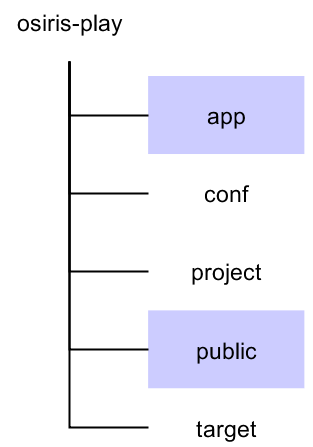
\includegraphics[height=60mm]{bilder/playapp.png}
\caption{Die Ordnerhierarchie der Anwendung. Blau markiert die besonders relevanten Ordner}
\label{fig:playapp}
\end{figure}

Bei der Programmierung wurde auf die Einhaltung der Clean Code-Prinzipien\footnote{\url{http://www.clean-code-developer.de/SOLID.ashx} (besucht am \today)}, wie beispielsweise \textit{DRY (Don't repeat yourself)} und \textit{SOC (Separation of Concerns)} geachtet. Aufgrund des Fehlens von Klassen in JavaScript, dem, im Gegensatz zu klassischen objektorientierten Sprachen, schwierigem Vererbungsmechanismus und der generell wünschenswerten Bevorzugung von Komposition vor Vererbung wurde für den Systementwurf das \textit{Flow Based Programming} (siehe Abschnitt \textit{Flow Based Programming}) eingesetzt. Für die SIRIS-Anbindung wurden Actors implementiert.

Die Module des Osiris-Renderers erfüllen alle eine spezielle Aufgabe und sind daher auch so benannt, beispielsweise \textit{DownloadSceneFromServer}. Alle Komponenten laufen asynchron und melden ihre Ergebnisse oder aufgetretene Fehler über registrierbare Callbacks als Ausgänge zurück. Dies verringert die Kopplung und erhöht die Wiederverwendbarkeit in anderen Projekten. Für die Rückgabe von Ergebnissen oder Fehlern wird in jedem Modul nur ein Callback registriert. Dies folgt der in AsyncJs vorgegebenen Form. Der erste Parameter ist immer ein etwaig aufgetretener Fehler oder \texttt{null}, wenn kein Fehler aufgetreten ist. Der zweite Parameter ist das Ergebnis. So ist es auch im NodeJS-Anwendungsframework\footnote{\url{http://nodejs.org/} (besucht am \today)} für welches AsyncJs ursprünglich entwickelt wurde.

Sowohl SIRIS als auch das Play! Framework verwenden zur Kompilation \textit{SBT (Simple Build Tool)}. Dies ist ein Werkzeug um die Erstellung von Scala-Projekten zu steuern, ähnlich wie \textit{Maven} oder \textit{Ant} für Java. Hierdurch konnte das SIRIS-Projekt Osiris einfach als Abhängigkeit hinzugefügt werden. Dadurch können in Osiris die SIRIS-Klassen importiert werden und bei der Kompilierung werden beide Projekte erstellt, zuerst SIRIS dann Osiris. Listing \ref{lst:osirissbtconfig} zeigt die Festlegung der Abhängigkeit.
\lstset{language=Scala}
\begin{lstlisting}[caption={Beschreibung der Abhängigkeit Osiris' von SIRIS in SBT}, label={lst:osirissbtconfig}]
lazy val siris = RootProject(file("../siris"))

val main = PlayProject(appName, appVersion, appDependencies, mainLang = SCALA).settings() dependsOn(siris) // Osiris depends on Siris
\end{lstlisting}

\section{Start von Osiris}
Beim Start der Anwendung wird zuerst der Jetty Server gestartet, auf dem das Play! Framework läuft. Darin werden die Controller für HTTP- und WebSocket-Requests, sowie die benötigten Actors für die SIRIS-Anbindung und die benötigten SIRIS-Actors selbst instanziiert.

Wenn der Benutzer nach dem Start der Anwendung die Url \texttt{http://localhost:9000} mit seinem Browser besucht, wird der Request an den \textit{Application}-Controller geleitet. Dieser erfüllt nun drei Aufgaben:
\begin{enumerate}
    \item Laden der Informationen zu den verfügbaren Shaderprogrammen
    \item Laden der Informationen zu den verfügbaren Szenen
    \item Einfügen der geladenen Informationen in das View-Template
\end{enumerate}
Die Informationen zu den verfügbaren Shaderprogrammen und Szenen finden sich in zwei vordefinierten JSON-formatierten Dateien, die im Dateisystem auf Serverseite liegen. Diese enthalten Metainformationen, wie Namen der Szenen und Shaderprogramme, die Pfade, wo die tatsächlichen Quelldateien gefunden werden können und im Falle der Shaderprogramme auch die bindbaren Attributes und Uniforms, mehr dazu etwas später. Diese Informationen werden gelesen, geparst, in das View-Template eingebaut und die fertige HTML-Seite anschließend an den Client ausgeliefert.

Alternativ zur Ablage im Dateisystem wäre der Einsatz einer dedizierten Datenbank möglich gewesen, welche die Informationen enthält. Der Einfachheit halber wurde jedoch hierauf verzichtet.

Sobald die HTML-Seite vom Client empfangen wurde, werden die verlinkte CSS-Datei und RequireJs geladen, welches seinerseits die im \texttt{data-main}-Attribut der HTML-Seite referenzierte Datei \textit{main.js} lädt und parst. In dem an \texttt{require.\-config} übergebenen anonymen Objekt befinden sich alle relevanten Informationen für RequireJs, um die Abhängigkeiten der benötigten Module aufzulösen und diese dann asynchron herunterzuladen. Im Anschluss wird das Modul \textit{Osiris} geladen und dessen \texttt{init}-Methode aufgerufen. Dieses Modul übernimmt nun drei Aufgaben:
\begin{enumerate}
    \item Initialisierung der Anwendung
    \item Kontrolle über das die grafischen Benutzeroberfläche manipulierende Viewmodel 
    \item Delegation der Anwendereingaben
\end{enumerate}
Das Layout und der Stil der grafischen Benutzeroberfläche werden in der HTML-Datei, respektive der \textit{main.css} festgelegt. Um jedoch eine klare Trennung von Layout/Stil und Anwendungscode zu erhalten, wurde ein separates Modul namens \textit{MainViewModel.js} im Ordner \textit{view} implementiert, welches sich an die HTML-Elemente anbindet und Funktionen bereitstellt um mit diesen zu interagieren. Für eine browserunabhängige Anbindung wurden die Möglichkeiten der \textit{Zepto}-Bibliothek verwendet. Diese bietet komfortable Methoden um HTML-Elemente zu manipulieren oder Informationen zu extrahieren. Das ViewModel stellt sowohl die vom \textit{Application}-Controller in die HTML-Seite eingefügten Shaderprogramm- und Szeneninformationen über die beiden Methoden \texttt{getCurrentShader} und \texttt{getCurrentScene}, als auch den Canvas für das Rendering über \texttt{getRenderCanvas} zur Verfügung. Zudem enthält die Seite einen Bereich für Statusmeldungen, über den die Applikation den Anwender über zur Laufzeit anfallende Benachrichtigungen und Fehler informieren kann. Den Zugriff hierauf abstrahiert das ViewModel über die Methode \texttt{updateStatus}.

Nachdem der Anwender nun die gewünschte Szene und das gewünschte Shaderprogramm gewählt und mit einem Klick auf den \textit{Start}-Button bestätigt hat, wird die \texttt{execute}-Methode des Osiris-Moduls aufgerufen.

\section{Initialisierung des WebGL-Kontext}
Der WebGL-Kontext ist inherent wichtig für fast alle Vorgänge innerhalb der Anwendung. Daher wird dieser zuerst initialisiert. Wie bereits beschrieben ist der Name des Kontexts noch nicht in allen Browsern auf "`webgl"' standardisiert, weshalb hierfür die WebGL Utils-Bibliothek angewendet wird. Listing \ref{lst:webglkontextaufbauen} zeigt den Aufruf innerhalb des Osiris-Moduls \textit{SetupWebGlContext}.
\lstset{language=JavaScript}
\begin{lstlisting}[caption={Initialisierung des WebGL-Kontext}, label={lst:webglkontextaufbauen}]
var glContext = WebGl.setupWebGL(canvas);
\end{lstlisting}
Da der Kontext für die Anwendung verloren gehen kann wird in allen Modulen, die auf den ihn angewiesen sind, vor der weiteren Verarbeitung die Funktion \texttt{isContextLost} aufgerufen. Es ist möglich über einen EventListener auf den Verlust des Kontexts zu reagieren. Allerdings schlugen Versuche hierzu fehl, da das Event kurioserweise immer direkt auftrat und so die Anwendung nicht weiterarbeiten konnte und andererseits jedes Modul anders auf den verlorenen Kontext reagieren muss. Es konnte auch nach einer längeren Recherche nicht nachvollzogen werden, warum das Event sofort geworfen wurde.

\section{Laden des gewählten Shaderprogramms}
Auf Clientseite wird das Modul \textit{LoadShaderProgram} gestartet, welches die Shaderinformationen des vom Anwender gewählten Shaderprogramms verarbeitet und über das registrierte Callback das fertige Shaderprogramm-Objekt zurückliefert. Zu den Shaderinformationen gehören der Name des Shaderprogramms, sowie Name und relativer Pfad zu einer Konfigurationsdatei. Letztere enthält folgende Daten:
\begin{itemize}
    \item Name der Datei, die den Code des Vertexshaders enthält
    \item Name der Datei, die den Code des Fragmentshaders enthält
    \item Bindbare Attributes und Uniforms
\end{itemize}
Für das Abrufen der nötigen Daten des gewählten Shaderprogramms existiert auf der Serverseite ein eigener Controller namens \textit{ShaderController}. Zuerst sendet der Client die JSON-enkodierten Informationen an den Server. Der ShaderController empfängt die Nachricht, lädt die referenzierte Konfigurationsdatei, parst sie und lädt die darin referenzierten Quellcodedateien für die Shader. Diese Informationen werden dann in ein JSON-Objekt verpackt und an den Client zurückgesendet. Dieser hat nun alle benötigten Daten um das gewählte Shaderprogramm zu erstellen. Hierfür müssen zuerst die beiden Shader kompiliert und dann dem Programm hinzugefügt werden. Schlussendlich wird das Programm noch "`gelinkt"'. Linken ist C-Programmierern ein Begriff. Nach der Kompilierung müssen die einzelnen Bestandteile noch zu einer ausführbaren Datei verbunden werden. Ähnlich gilt dies auch für ein WebGL-Shaderprogramm. Damit das Programm schlussendlich verwendet werden kann, wird die Funktion \texttt{useProgram} mit dem gelinkten Shaderprogramm als Parameter aufgerufen.

\section{Laden der gewählten Szene}
Das Laden der vom Anwender gewählten Szene läuft ähnlich ab wie das Laden des Shaderprogramms. So werden auch hier die Informationen zur gewählten Szene an einen dedizierten Controller namens \textit{SceneController} übertragen, welcher dann die Szene selbst zurückgibt. Jedoch müssen zuerst einige der enthaltenen Knoten in ein für den Renderer verständliches Format umgewandelt und referenzierte Daten, wie 3D-Modelle und Texturen, nachgeladen und ihrerseits transformiert werden.

\subsection{3D-Modelle}
WebGL benötigt die modellrelevanten Daten, wie Vertices, Normalen oder Indizes als strikt typisierte Bufferobjekte. Daher wurden in JavaScript typisierte Array-Objekte (siehe \autocite{TypedArrays}) eingeführt, welche nur einen bestimmten Datentypen enthalten können, wie das \textit{Float32Array} oder das \textit{Uint16Array}. WebGL stellt zwei binäre Bufferobjekte bereit, AR\-RAY\-\_BUF\-FER und EL\-E\-MENT\-\_AR\-RAY\-\_BUF\-FER. Deren Inhalte können über diese typisierten Arrays manipuliert werden. Die typisierten Arrays fungieren hier als "`Sicht"' (View) auf den Buffer. Da dieser immer nur binäre Daten enthält, wird durch das Array beschrieben welche Art von Daten sich darin befinden.

Alle für das Rendering relevanten Daten müssen in WebGL-Bufferobjekte umgewandelt werden, wie Listing \ref{lst:webglbuffer} zeigt.
\lstset{language=JavaScript}
\begin{lstlisting}[caption={Erstellen eines WebGL-Buffers und Anbinden der Daten}, label={lst:webglbuffer}]
var buffer = _gl.createBuffer();
_gl.bindBuffer(_gl.ARRAY_BUFFER, buffer);
_gl.bufferData(_gl.ARRAY_BUFFER, new Float32Array(vertices), _gl.STATIC_DRAW);
_gl.bindBuffer(_gl.ARRAY_BUFFER, null);
\end{lstlisting}
Zuerst wird ein Bufferobjekt erstellt, dann als ARRAY\-\_BUFFER-Typ referenziert und anschließend über ein Float32Array mit Daten befüllt. In der letzten Zeile wird die Referenz auf den Buffer gelöst, um ungewollte Veränderungen zu vermeiden.
\begin{figure}
\centering
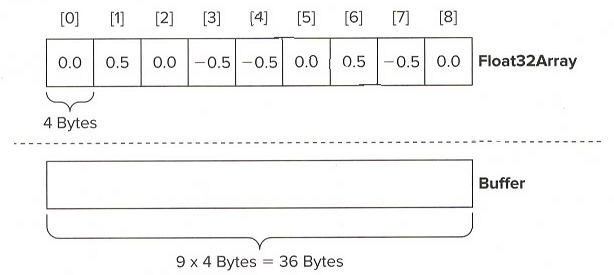
\includegraphics[width=100mm]{bilder/vbo.png}
\caption{Ein Bufferobjekt (unten) und die Float32Array-Sicht auf diesen Buffer (oben) \autocite{WebGlPogramming}}
\label{fig:vbo}
\end{figure}

\subsection{Texturen}
In der Szene werden Texturen als JPEG- oder PNG-Bilder referenziert. Diese können nicht direkt in WebGL verwendet werden sondern müssen zuerst umgewandelt werden. Dies ist mit Hilfe des in JavaScript vorhandenen \textit{Image}-Objekts sehr schnell umsetzbar. Dieses lädt die referenzierten Bilddateien asynchron herunter, was die gleichzeitige Verarbeitung mehrerer Bilder ermöglicht und somit die Vorbereitungszeit für das Rendering verkürzt. Über den in Listing \ref{lst:jsimageladen} gezeigten Code wird ein Bild von der angegeben Adresse heruntergeladen.
\lstset{language=JavaScript}
\begin{lstlisting}[caption={Herunterladen eines Bildes mit dem JavaScript Image-Objekt}, label={lst:jsimageladen}]
var image = new Image();

image.onload = function() {
  _handleLoadedImage(image, callback);
};

image.src = pathToImage;
\end{lstlisting}
Im \texttt{\_handleLoadedImage}-Callback wird dann die Erstellung einer WebGL-Textur durchgeführt. Listing \ref{lst:imageintextur} zeigt den Vorgang.
\lstset{language=JavaScript}
\begin{lstlisting}[caption={Umwandlung eines Image-Objekts in eine WebGL-Textur}, label={lst:imageintextur}]
function _handleLoadedImage(image, callback) {
  var texture = _gl.createTexture();

  _gl.bindTexture(_gl.TEXTURE_2D, texture);
  _gl.pixelStorei(_gl.UNPACK_FLIP_Y_WEBGL, true);
  _gl.texImage2D(_gl.TEXTURE_2D, 0, _gl.RGBA, _gl.RGBA, _gl.UNSIGNED_BYTE, image);
  _gl.texParameteri(_gl.TEXTURE_2D, _gl.TEXTURE_MAG_FILTER, _gl.LINEAR);
  _gl.texParameteri(_gl.TEXTURE_2D, _gl.TEXTURE_MIN_FILTER, _gl.LINEAR_MIPMAP_LINEAR);
  _gl.generateMipmap(_gl.TEXTURE_2D);

  _gl.bindTexture(_gl.TEXTURE_2D, null);

  callback(null, texture);
}
\end{lstlisting}
Zuerst wird eine WebGL-Textur erstellt, die Referenz darauf in der Variable \texttt{texture} gespeichert und als aktuell zu bearbeitende Textur gebunden. Der Aufruf der Funktion \texttt{pixelStorei(\_gl.UNPACK\-\_FLIP\-\_Y\-\_WEBGL, true)} dreht das Bild horizontal, da der Koordinatenursprung des Image-Objekts in der linken oberen Ecke, bei einer WebGL-Textur in der linken unteren Ecke liegt (siehe Abbildung \ref{fig:bilderkoordinatensysteme}).

Anschließend werden die Bytes des Bildes von der Funktion \texttt{texImage2D} aus dem Image-Objekt gelesen. Hierbei ist es wichtig anzugeben welche Farbkanäle das Bild enthält (RGB: Rot, Grün und Blau) und ob das Bild Transparenzen enthalten kann (Das A in RGBA steht für den Alphakanal). Für die visuelle Qualität sind zudem die Angaben für die Filterung der Textur notwendig. In diesem Beispiel wird die \textit{trilineare} Filterung verwendet. Um die Darstellungsqualität und die Leistung zu verbessern, können Mipmaps generiert werden (Funktion \texttt{generateMipmap}). Dies sind verkleinerte Repräsentationen des Originalbildes. Mit steigender Entfernung vom Betrachter zur Textur wird auf eine höhere Mipmapstufe umgeschaltet und nur noch das verkleinerte Abbild gezeichnet. Allerdings ist bei der Verwendung von Mipmaps zu beachten, dass die Größe der Textur dann ein Vielfaches von 2 sein muss (2, 4, 8, 16, 32 etc.). Höhe und Breite können sich unterscheiden (zum Beispiel: 128x512 Pixel). Am Ende des Beispiels wird über den erneuten Aufruf von \texttt{bindTexture} die Referenz auf die aktuelle Textur gelöst, um weitere Änderungen zu vermeiden.
\begin{figure}
\centering
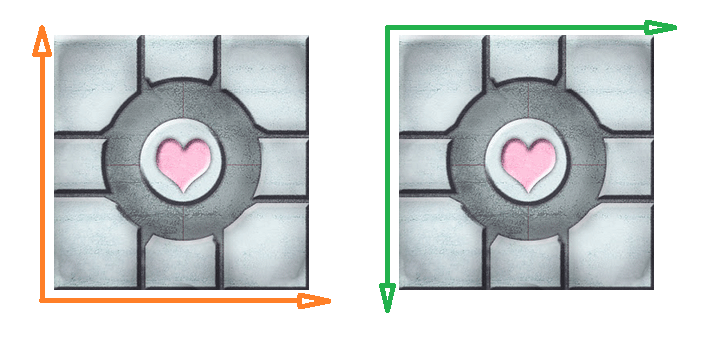
\includegraphics[width=\textwidth]{bilder/koordinatensysteme_bilder.png}
\caption{Links: Das Koordinatensystem einer WebGL-Textur, Rechts: Das Koordinatensystem des JavaScript Image-Objekts}
\label{fig:bilderkoordinatensysteme}
\end{figure}

Um die Texturen anzeigen zu können muss das 3D-Modell über Texturkoordinaten verfügen. Diese liegen wie bereits von OpenGL gewohnt zwischen 0 und 1. Für jedes Vertex wird ein Zweiertupel angegeben.

Osiris unterstützt zwei Texturtypen: Color Maps und Specular Maps (siehe Abbildung \ref{fig:texturemaps}). Color Maps enthalten die Farbinfomartionen, Specular Maps den Grad der Reflektivität für jedes Pixel. Je dunkler ein Pixel, desto weniger stark reflektiert das Licht an diesem Punkt. Weiß würde also volle Reflektion bedeuten, Schwarz gar keine.
\begin{figure}
\centering

\includegraphics[width=\textwidth]{bilder/texturemaps.png}
\caption{Links: eine Color Map, Rechts: die zugehörige Specular Map}
\label{fig:texturemaps}
\end{figure}

Hierbei ist zu beachten, dass alle Modellknoten die gleichen Arten von Texture Maps haben. Referenziert beispielsweise ein Modellknoten eine Specular Map in seinen Materialeigenschaften, sollten alle Modellknoten eine Specular Map referenzieren. Ansonsten kann es zu visuellen Artefakten kommen.

\section{Übertragen der Modellknoten an SIRIS}
Der Renderer sucht alle Modellknoten aus der Szene und sendet sie an den Server, welcher sie über die Anbindung an SIRIS der ebenfalls angebundenen Physikengine zugänglich macht. Für diese sind im Modellknoten seine physikalischen Eigenschaften, wie Masse, Reibungswiderstand, sowie Form und Größe der physikalischen Hüllform hinterlegt. Weiterhin benötigt die Physikengine die Transformationsmatrix des Objekts. Diese bestimmt sowohl die Position, als auch die Ausrichtung (Rotation) des Modells. Die Physikengine errechnet die physikalischen Kräfte, die auf das Objekt einwirken und aktualisiert dessen Transformationsmatrix. Der Renderer verwendet sie um das Objekt dann in der korrekten Position und Ausrichtung zu zeichnen.

\subsection{Vorbereitung der Datenübertragung}
Der Renderer extrahiert die Modellknoten über die Methode \texttt{byType} des Moduls \textit{FindNodes}. Diese liefert alle Knoten des Szenegraphen mit dem angegebenen Typen zurück, in diesem Fall mit dem Typen "`model"'.

Da die Kommunikation mit dem Server zu keinen unerwarteten Ergebnissen führen soll, wurden vorgefertigte Nachrichtentypen erstellt. Diese wandeln die über die Konstruktorparameter übergebenen Daten in eine vordefinierte JSON-Struktur um. Der Renderer kann zwei Nachrichtentypen an den Server senden:
\begin{enumerate}
    \item \textbf{SetupRequest}\\
Dient dem Senden von Modelknoten an SIRIS, für die es Entitäten erstellen und registrieren soll. Weiterhin sollen Veränderungen der Transformationsmatritzen der einzelnen Knoten überwacht und dem Renderer mitgeteilt werden. Als Parameter wird ein Array mit den Modelknoten erwartet. Ist für einen der Knoten bereits eine Entität registriert, wird dessen Transformationsmatrix durch die des übermittelten Knoten ersetzt. Dies ist beispielsweise eine Möglichkeit bereits registrierte Entitäten auf ihre ursprüngliche Position und Ausrichtung zurückzusetzen.
    \item \textbf{ManipulationRequest}\\
Dient der Mitteilung an SIRIS, dass eine registrierte Entität auf eine bestimmte Art und Weise manipuliert werden soll. Als Parameter werden die ID des Knoten, die Art der Manipulation (derzeit lediglich \textit{ApplyImpulse}) und die nötigen Manipulationsdaten (für \textit{ApplyImpulse} ein Array mit dem dreiteiligen Impulsvektor) erwartet.
\end{enumerate}

\subsection{Datenübertragung}
Die gesamte Kommunikation mit dem Server läuft über das Modul \textit{SendMessageToServer}. Es abstrahiert die API des WebSockets und bietet ein Callback an, über das andere Module sich über Antworten benachrichtigen lassen können. Das Callback wird bei jedem Aufruf ersetzt um zu verhindern, dass Module die sich bereits früher registriert haben keine Nachrichten mehr empfangen, wenn ihre Arbeit bereits getan ist. Die Verbindung wird aber nur ein Mal beim ersten Senden aufgebaut.

Das WebSocket verbindet sich auf Serverseite mit dem \textit{OsirisController}. Die Nachrichten werden hier angenommen und an den Actor \textit{OsirisMessageEvaluator} übergeben. Da die Nachrichten standardisiert sind kann dieser die Eigenschaft \texttt{request} auslesen, daraufhin die Nachricht in den äquivalenten Scala-Nachrichtentyp umwandeln und diesen an den Actor \textit{SirisOverlord} senden. Alle Nachrichten, die innerhalb der Osiris-Serverkomponente und zum Client verschickt werden können, sind ebenfalls standardisiert. Ihre Definitionen befinden sich in den Traits \textit{OsirisInternalMessage} und \textit{OsirisResponseMessage} des \textit{osiris.contracts}-Package.

\subsection{Registrieren der Entitäten in SIRIS}
SirisOverlord ist ein SIRIS-Actor. Er steuert einerseits die Registrierung und Manipulation der vom Renderer gesendeten Modellknoten und benachrichtigt den Renderer über den OsirisMessageEvaluator über Veränderungen der Transformationsmatritzen der registrierten Entitäten. Hierzu bedient er sich der bereits im Abschnitt \textit{SIRIS} des Kapitels \ref{chap:technologien} beschriebenen Methoden von SIRIS. In Listing \ref{lst:entitycreatregister} wird der Ablauf bei einem eingehenden \textit{SetupRequest} gezeigt.
\lstset{language=Scala}
\begin{lstlisting}[caption={Erzeugen und Registrieren einer neuen Entität}, label={lst:entitycreatregister}]
msg.nodes foreach {
  node => {
    val id = Symbol((node \ "id").as[String])

    handleEntity(id)(entity => entity match {
      case Some(ent) => physicsActor ! SetTransformation(ent, _makeTransformation(node))
      case None => {
        realize(
          EntityDescription(
            _makePhysicShape(node)
          ),
          (e: Entity) => {
            registerEntity(id, e)

            e.get(Transformation) match {
              case Some(sVar) => observe(sVar, (mat: Mat4x4) => origin ! TransformRequest(id.name, FloatMath.transpose(mat)))
              case None => origin ! OsirisError("The node '" + id + "' has no transformation")
            }
          }
        )
      }
    })
  }
}

origin ! NodesSetupComplete()
\end{lstlisting}
Für jeden Knoten wird zuerst über die Methode \texttt{handleEntity} nachgesehen, ob unter der Knoten-ID bereits eine Entität registriert ist. Hierfür wird das Scala-Sprachfeature des \textit{Pattern Matching} verwendet. Falls ja (\texttt{case Some(ent)}) wird der Physik-Actor angewiesen deren Transformationsmatrix durch die des Knotens zu ersetzen. Andernfalls (\texttt{case None}) ist noch keine Entität mit dieser ID registriert. \texttt{\_makeTransformation} ist eine Hilfsmethode, um das Transformationsarray in den benötigten Datentypen umzuwandeln. Sollte jedoch unter dieser ID noch keine Entität registriert sein, wird mit der bereits in Abschnitt \textit{SIRIS} beschriebenen \texttt{realize}-Methode eine \textit{EntityDescription} erstellt. Der einzige Aspekt der hierbei von Interesse ist, ist die physikalische Hüllgeometrie. Deren Erstellung übernimmt die Hilfsmethode \texttt{\_makePhysicShape}.

Sobald die Entität erstellt wurde, wird das registrierte Callback aufgerufen. Dieses registriert die Entität über \texttt{registerEntity} und registriert seinerseits mittels der Methode \texttt{observe} ein Callback, welches auf die Veränderung der Transformationsmatrix der Entität reagiert und in diesem Falle einen \textit{TransformRequest} an den OsirisMessageEvaluator schickt.

An dieser Stelle noch eine Anmerkung zum \textit{TransformRequest}. Der Physik-Actor liefert die Transformationsmatrix in der \textit{Row Major-Form}, WebGL benötigt jedoch die \textit{Column Major-Form}. Diese entspricht der transponierten Row Major-Matrix. Abbildung \ref{fig:rowcolumn} zeigt auf der linken Seite eine Row Major-Matrix, rechts die Transponierte. Diese entspricht der Darstellungs als Column Major-Matrix. Die Transformationsmatrix jedes Knotens besteht aus den in Abbildung \ref{fig:transformationsmatrix} dargestellten Anteilen. Aus den vorgenannten Gründen wird die zurückgelieferte Matrix vorher transponiert.
\begin{figure}
\centering
\[
\begin{pmatrix}
1 & 2 & 3 & 4\\
5 & 6 & 7 & 8\\
9 & 10 & 11 & 12\\
13 & 14 & 15 & 16
\end{pmatrix}
=
\begin{pmatrix}
1 & 5 & 9 & 13\\
2 & 6 & 10 & 14\\
3 & 7 & 11 & 15\\
4 & 8 & 12 & 16
\end{pmatrix}^T
\]
\caption{Links: Row Major-, Rechts: Column Major-Matrix (Transponierte Row Major)}
\label{fig:rowcolumn}
\end{figure}
\begin{figure}
\centering
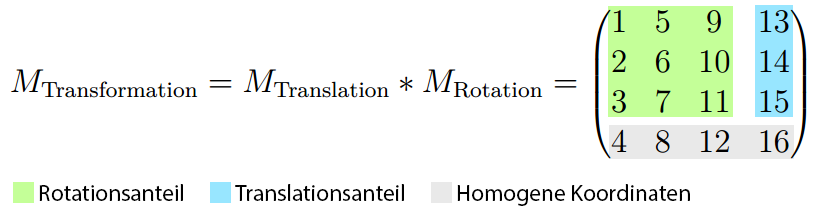
\includegraphics[width=120mm]{bilder/transformationsmatrix.png}
\caption{Bestandteile der homogenisierten Transformationsmatrix}
\label{fig:transformationsmatrix}
\end{figure}

Der Server wandelt den TransformRequest in eine JSON-Struktur um und sendet diese über das Socket zurück an den Client. Sobald alle Knoten durchlaufen wurden, sendet der SirisOverlord die Nachricht \textit{NodeSetupComplete} an den OsirisMessagEvaluator zurück, welcher diese in ein JSON umwandelt und an den Client schickt. Der Client registriert dies und fährt mit der Vorbereitung für das Rendering fort.

\section{Benutzereingaben verarbeiten}
Über die Tastatur soll der Benutzer mit der Szene interagieren können. Da Szenen sehr unterschiedlich aufgebaut sein können, muss in der Szene hinterlegt sein welche Tastendrücke was bewirken. Zu diesem Zweck wurde in der Szene ein Knoten vom Typ "`keyboard"' hinterlegt, welcher die aktivierbaren Tasten und die daraufhin auszuführenden Aktionen in einer Keymap beschreibt. Das hierfür notwendige Modul heißt \textit{HandleUserInput}. Um die Modellknoten verändern zu können, müssen innerhalb des Moduls Referenzen auf diese vorgehalten werden. Zudem verwendet es das \textit{SendMessageToServer}-Modul, um die auszuführenden Aktionen (derzeit nur \textit{ApplyImpulse}) an den Server schicken und die Antworten verarbeiten zu können. Listing \ref{lst:userinput} zeigt den Code um auf Benutzereingaben reagieren zu können. Das \texttt{\$}-Zeichen ist die Factory-Methode der \textit{Zepto}-Bibliothek.
\lstset{language=JavaScript}
\begin{lstlisting}[caption={Reaktion auf Benutzereingaben}, label={lst:userinput}]
$(document).keydown(function(event) {
  var manipulationRequest = node.keyMap[event.which];

  if (manipulationRequest) {
    SendMessage.execute(new Msg.ManipulationRequest(manipulationRequest.nodeId, manipulationRequest.type, manipulationRequest.data), _onServerResponse);
  }
});
\end{lstlisting}
Wenn der Anwender eine Taste drückt die eine Aktion hervorrufen soll, wird mit den in der Keymap hinterlegten Daten ein neuer \textit{ManipulationRequest} erzeugt und an den Server gesendet. Listing \ref{lst:transformrequest} zeigt den Ablauf bei einer Antwort des Servers.
\lstset{language=JavaScript}
\begin{lstlisting}[caption={Reaktion auf Benutzereingaben}, label={lst:transformrequest}]
var nodeToTransform;

if (response.status === "transform") {
  nodeToTransform = _nodesToHandle[response.data.nodeId];
  nodeToTransform.transformation = response.data.transformation;
}
\end{lstlisting}
Bei einer gültigen Antwort (der Status ist "`transform"') wird der zu transformierende Modellknoten über die zurückgelieferte ID in der Map \texttt{\_nodesToHandle} gesucht. Anschließend wird seine gegenwärtige Transformationsmatrix durch die in der Servernachricht enthaltene ersetzt.

\section{Darstellen der Szene}
Vor dem Rendering muss festgelegt werden welche Daten mit welchem Zweck an das Shaderprogramm gebunden werden. Dieses Binden ist notwendig, da weder der Renderer noch das Shaderprogramm wissen können, ob und wie die in der Szene enthaltenen Daten mit den Attributes und Uniforms in den Shadern assoziiert sind. Wie bereits beschrieben enthält die vom Server zurückgelieferte Shaderprogrammkonfiguration auch Informationen über die bindbaren Attributes und Uniforms. Das Modul \textit{SetupShaderBindableLocations} sucht diese im Shaderprogramm und speichert ihre Referenzen in einem \texttt{locations}-Objekt. Dies wird später in der Rendering-Schleife verwendet um relevante Daten, wie die Vertices eines 3D-Modells oder Texturinformationen, an die Shader zu übertragen. Im Modul \textit{RenderScene} wird anschließend die Rendering-Schleife ausgeführt. In WebGL kann hierfür die Funktion \texttt{requestAnimationFrame} verwendet werden, welche für jedes gerenderte Bild aufgerufen wird. Diese Funktion bietet zudem noch einige Komfortfunktionen. Sollte der aktuelle Tab oder Fenster beispielsweise nicht mehr sichtbar sein weil der Benutzer einen anderen Tab oder Fenster geöffnet hat, wird die Animationsschleife nicht mehr ausgeführt. Dies reduziert die Belastung der Hardware und spart Energie. Der Browser kann noch weitere Optimierungen vornehmen, je nachdem wie der Browserhersteller die Funktion implementiert hat. Da der Name der Funktion noch nicht in allen Browser standardisiert ist, wurde auch hierfür die WebGL Utils-Bibliothek verwendet.
\begin{figure}
\centering
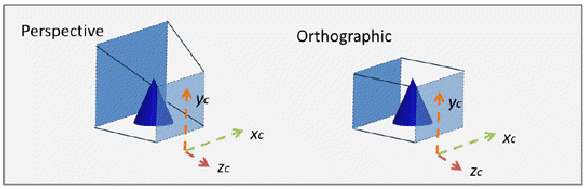
\includegraphics[width=\textwidth]{bilder/views.png}
\caption{Links: der kegelförmige Sichtraum der Perspektivischen Projektion, Rechts: der quaderförmige Sichtraum der Orthographischen Projektion\autocite{WebGLBeginnersGuide}}
\label{fig:views}
\end{figure}

Zur Darstellung der Szene verwendet der Renderer zwei Matritzen:
\begin{enumerate}
    \item \textbf{Modelviewmatrix}\\
Die Modelviewmatrix ist die kombinierte Matrix aus der Model- (3D-Objekt) und der Viewtransformation (Kamera) in der Szene. Sie bestimmt die Position und Ausrichtung jedes Objekts in der Szene und ist daher von besonderer Bedeutung.
    \item \textbf{Projektionsmatrix}\\
Die Projektionsmatrix bestimmt wie die Szene dargestellt wird. Hierzu sind zwei Projektionsarten möglich: In der Orthographischen Projektion bleiben parallele Linien parallel und Objekte behalten, unabhängig von ihrer Entfernung zum Betrachter, ihre proportionale Größe. In der Perspektivischen Projektion hingegen werden Objekte die vom Betrachter weiter entfernt sind kleiner gezeichnet. Die Perspektivische Projektion ergibt ein realitätsgetreueres Bild.
\end{enumerate}
Auf die Relevanz dieser Matrizen wird weiter unten bei der Beschreibung der Vorgänge für jeden Knoten näher eingegangen.
\lstset{language=JavaScript}
\begin{lstlisting}[caption={Implementierung der Lookup-Tabelle für das Rendering}, label={lst:lookuptable}]
var _lookupTable = {
  "renderInformation": _updateRenderer,
  "camera": _updateViewport,
  "ambientLight": _updateAmbientLight,
  "pointLight": _updatePointLight,
  "model": _renderModel
};
\end{lstlisting}
Da der gesamte Rendering-Vorgang recht komplex ist wurde hierfür ein extra Modul namens \textit{TraverseAndRender} hinzugefügt. In jeder Iteration der Renderschleife wird die Szene darin einmal traversiert und je nach gefundenem Knotentyp gehandelt. Die Traversierung erfolgt rekursiv. Für jeden gefundenen Knoten wird ein registriertes Callback ausgeführt. Das Callback entscheidet dann anhand des Knotentypen wie mit diesem verfahren werden muss. Um längere Entscheidungsbäume und damit potenzielle Leistungseinbußen zu vermeiden wurde hierfür eine Lookup-Tabelle verwendet (siehe Abbildung \ref{fig:lookupvergleich}).
\begin{figure}
\centering
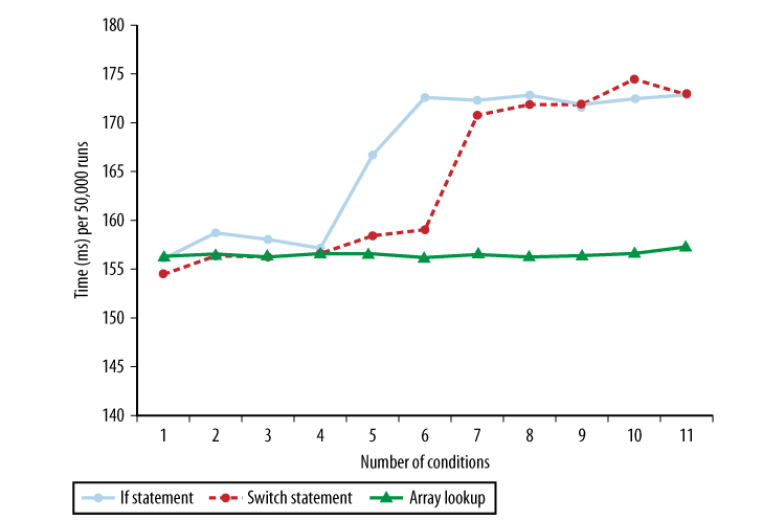
\includegraphics[width=\textwidth]{bilder/lookup_vergleich.png}
\caption{Leistungsvergleich Lookup-Table, If-Else und Switch im IE 7 \autocite{HighPerformanceJS}}
\label{fig:lookupvergleich}
\end{figure}
Diese ist ein einfaches JavaScript-Objekt, in dem der Knotentyp die auszuführende Funktion referenziert (siehe Listing \ref{lst:lookuptable}).
Sobald der gefundene Knotentyp in der Lookup-Tabelle gefunden wurde, wird die dort referenzierte Funktion ausgeführt. Für die folgenden Knoten sind Funktionen registriert.

\subsection{Modellknoten}
Für jeden Modellknoten wird versucht mindestens die Vertices und Indizes im Vertexshader zu binden, da diese die Mindestanforderung darstellen um das Modell zeichnen zu können. Indizes definieren die Faces (Oberflächen) des 3D-Modells explizit, indem sie die Reihenfolge der zu zeichnenden Dreiecke angeben. Andere Rendermodi als \texttt{TRIANGLES} werden vom Renderer nicht unterstützt. Sollten jedoch weitere Informationen, wie die Normalen, Texturkoordinaten, Texturen etc. vorhanden sein, werden diese ebenfalls über die im \texttt{locations}-Objekt enthaltenen Referenzen an ihre jeweiligen Attributes bzw. Uniforms angebunden.

Um zu garantieren, dass jedes Modell in der Szene später unabhängig von anderen Objekten gezeichnet wird und nur auf es einwirkende physikalische Kräfte reagiert, wird vor dem Zeichnen eine Kopie der aktuelle Modelviewmatrix auf einem Stack abgelegt. Die originale Modelviewmatrix wird mit der aktuellen Transformationsmatrix des Objekts multiplitziert, wodurch das Objekt genau an der Position und mit der Ausrichtung gezeichnet wird, die von seiner Transformationsmatrix vorgegeben wird. Nach dem Zeichenvorgang wird die originale Modelviewmatrix wieder vom Stack geladen und so verhindert, dass die Transformation des vorherigen Objektes Einfluss auf das nachfolgende hat.

In den Modellknoten können Materialeigenschaften wie \texttt{diffusecolor} oder Texturen hinterlegt werden. Je Knoten sind eine Color und eine Specular Map möglich.

\subsection{Kameraknoten}
Wie OpenGL ES hat auch WebGL kein dediziertes Kameraobjekt. Um ein solches zu simulieren ist die Projektionsmatrix von besonderer Bedeutung. Der Renderer unterstützt sowohl die Orthographische als auch die Perspektivische Projektion. Die Art der Projektion wird im "`camera"'-Knoten in der Szene eingestellt. Für das Einstellen der Projektionsart bietet die \textit{glMatrix}-Bibliothek die Hilfsfunktionen \texttt{perspective} und \texttt{ortho} an. Im Eigenschaftsobjekt \texttt{optics} des Kameraknotens werden die notwendigen Informationen, wie beispielsweise Öffnungswinkel, Near und Far Plane, erwartet.

Auch für das Festlegen der Position, des Blickziels und der Ausrichtung der Kamera bietet die \textit{glMatrix}-Bibliothek eine Hilfsfunktion namens \texttt{lookAt}. Die hierfür notwendigen Informationen sind im Eigenschaftsobjekt \texttt{position} des Kameraknotens hinterlegt (siehe auch Abbildung \ref{fig:cam}). Auf diese Weise lassen sich alle für die Kamera relevanten Informationen auf menschenlesbare Weise in der Szene hinterlegen.
\begin{figure}
\centering
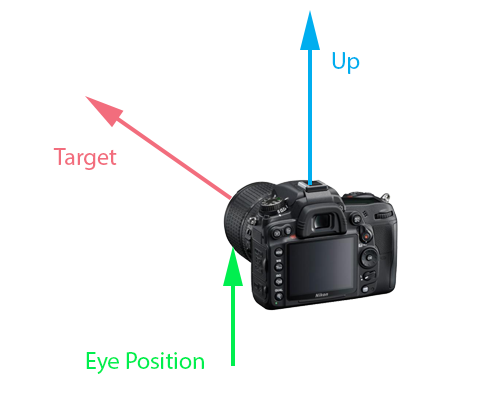
\includegraphics[width=80mm]{bilder/cam.png}
\caption{Relevante Vektoren der Kamera (Copyright des Kamerabildes: \copyright Nikon Corporation)}
\label{fig:cam}
\end{figure}
Damit der Rendering Canvas beim Vergrößern und Verkleinern des Browserfensters mitskaliert, wird die Größe des Canvas und das Ansichtsverhältnis bei jedem Durchlauf der Renderschleife neu berechnet.

\subsection{Renderinformationen}
Die für den Renderer relevanten Informationen werden im Knotentyp "`renderInformation"' hinterlegt. Hierzu gehören:
\begin{itemize}
    \item \textbf{Clear color}\\
Die RGB-Werte, mit denen der Color Buffer initial überschrieben wird.
    \item \textbf{Clear}\\
Die Buffer, die zurückgesetzt werden sollen. Dies muss als Integerwert angegeben werden. Die Buffer sind als Konstanten in WebGL hinterlegt, so ist der Wert für das \textit{COLOR\-\_BUFFER\-\_BIT} 16384. Sollen sowohl der Color Buffer als auch der Depth Buffer zurückgesetzt werden, ist der Wert 16640. Dies ist die Summe aus 16384 und 256 (\textit{DEPTH\-\_BUFFER\-\_BIT}) \autocite{WebGLSpec}.
\end{itemize}
Diese können somit beispielsweise über Anwendereingaben geändert werden, da sie in jedem Durchlauf der Renderschleife überprüft werden.

\subsection{Beleuchtungsknoten}
Der Renderer unterstützt die Festlegung der Werte für das ambiente Licht, sowie Punkt-, direktionale und Spotlichquellen. Die eigentliche Unterstützung hierfür muss natürlich im Shader eingebaut sein. Der Renderer weiß lediglich welche Daten für den jeweiligen Lichttyp mindestens benötigt werden und an das Shaderprogramm gesendet werden müssen. Es ist jeweils nur maximal ein Licht jeden Typs pro Szene verfügbar.
\chapter{Fazit und Ausblick}
Das Ziel dieser Arbeit war ein verteiltes 3D-Echtzeit-Renderingsystem zu entwicklen, dass in der Lage ist eine 3D-Szene mit Hilfe von WebGL auf dem Client darzustellen und an ein Realtime Interactive System angebunden ist. Hierzu wurden ein WebGL-Renderer, eine serverseitige Webanwendung auf Basis des Play! Frameworks und die Anbindung an ein bestehendes RIS vollständig neu implementiert.
\begin{figure}
\centering
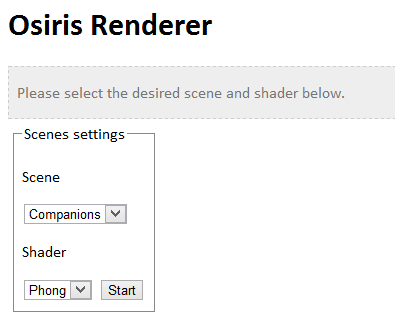
\includegraphics[width=90mm]{bilder/osirissettings.png}
\caption{Auswahl der zu rendernden Szene und des Shaderprogramms}
\label{fig:osirissettings}
\end{figure}

Die wesentliche Herausforderung war die Interaktion der unterschiedlichen Technologien untereinander sicher zu stellen, was eine intensive Einarbeitung in die einzelnen Wissensfelder erforderte.

Insbesondere die Anbindung an SIRIS, das verwendete RIS, gestaltete sich zuerst als schwierig da es bisher kaum dokumentiert ist. Im Endeffekt gestaltete sie sich nach der notwendigen Einarbeitungszeit in das System jedoch als überraschend einfach. Die Hauptaufgabe wird von einem SIRIS-Actor übernommen, der lediglich 148 Zeilen Quelltext lang ist. In kleinem Maßstab diente Osiris damit auch als Feldtest für die Entwicklung einer völlig neuartigen Komponente für das RIS.

Der WebGL-Renderer ist in der Lage vom Anwender gewählte Szenen mit unterschiedlichen Shaderprogrammen und dessen Interaktion mit den Objekten der Szene darzustellen und mit dem serverseitigen RIS zu kommunizieren. Allerdings muss auch festgesetllt werden, dass eine beliebige Kombination von Szenen und Shaderprogrammen nicht möglich ist. Der Renderer kann besipielsweise Szenen, die mehrere Lichtquellen eines Typs (mehrere Spotlichter beispielsweise) nicht darstellen. Da Shader völlig frei programmierbar sind, müsste hier deutlich mehr Aufwand betrieben werden, was jedoch im Rahmen dieser Arbeit weder Aufgabe noch zeitlich möglich gewesen wäre.

In der Planungsphase des Projekts gab es Bedenken, dass die Kommunikation zwischen dem clientseitigen Renderer und dem serverseitigen RIS nicht performant genug wäre, um eine Echtzeitinteraktion des Anwenders mit den Objekten der Szene und der Objekte untereinander zu realisieren. Letztendlich hat es sich jedoch herausgestellt, dass die Kommunikation mit (kleinen) JSON-Nachrichten über ein WebSocket zumindest für die derzeit in Osiris enthaltenen Szenen völlig ausreicht. Für eine realistische Einschätzung der Belastbarkeit und Leistungsfähigkeit wäre ein zukünftiger Performancetest mit sehr komplexen Szenen und vielen Objekten notwendig, welcher jedoch den zeitlichen Rahmen dieser Arbeit gesprengt hätte.
\begin{figure}
\centering
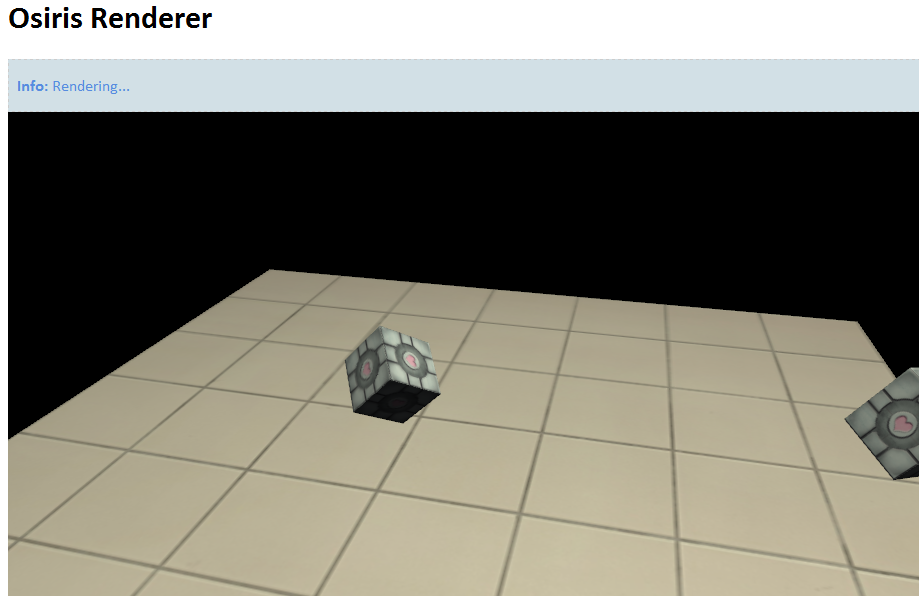
\includegraphics[width=\textwidth]{bilder/osiris.png}
\caption{Ein Bild des laufenden Renderers}
\label{fig:osiris}
\end{figure}

Die Wahl des Play! Frameworks als Grundlage für die serverseitige Webanwendung hat sich als sehr günstig erwiesen. Es bietet alle benötigten Strukturen an, ohne jedoch die Programmierung durch Konfigurationsaufwand oder umständliche Verwendung zu behindern. Tatsächlich waren die Controller für die statischen Ressourcen und die WebSocket-Verbindung sehr zeitnah implementiert. Aufgrund seiner Architektur und des statuslosen Zustands bei Anfragen ist es einerseits möglich Anwendungen ohne größeren Aufwand schnell zu skalieren und es, wenn gewünscht, auch relativ leicht durch eine andere Lösung zu ersetzen. Leider hat der statuslose Zustand aber auch einen Nachteil, nämlich den höheren Zeitaufwand der nötig gewesen wäre, um eine Mehrbenutzerumgebung zu implementieren. Osiris ist in seinem aktuellen Prototypenstatus lediglich von einem Benutzer verwendbar.

In der Nachschau hätten einige Aspekte mit mehr Zeit besser gelöst werden können. Von der Schlichtheit der Gui mal abgesehen wäre beispielsweise zur Flexibilisierung des Shaderprogramms ein System besser, welches nicht direkt von den Attributes und Uniforms abhängt, sondern einer abstrakten Beschreibung der erwarteten Darstellung. Diese würde gelesen und zur Laufzeit daraus dynamisch ein passendes Shaderprogramm generiert werden. Auch wäre zur Leistungssteigerung eine vollständigere Umwandlung der vom Server geladenen Szene in einen nur noch die relevanten Teile enthaltenden und auf Traversierungsgeschwindigkeit optimierten Szenegraphen und das Aufteilen der Renderschleife in verschiedene Renderpasses günstig gewesen. Zur nochmaligen Verkleinerung der zwischen Client und Server ständig übertragenen Datenmenge könnte zudem das MessagePack-Format\footnote{\url{http://msgpack.org/} (besucht am \today)} statt JSON verwendet werden. Jedoch wären diese Verbesserungen in der kurzen Zeitspanne der Bachelorarbeit allein kaum möglich gewesen. Sie eröffnen jedoch Möglichkeiten auf dem gewonnenen Wissen aufzubauen.

Zusammenfassend kann die gestellte Aufgabe als vollständig gelöst betrachtet werden. Im Endergebnis konnte gezeigt werden, dass es durch die Verwendung von WebGL und der Anbindung an ein serverseitiges RIS möglich ist, 3D-Anwendungen zu entwickeln, die keine besonderen Anforderungen benötigen. Ein aktueller Browser wie Google Chrome oder Mozilla Firefox reicht völlig aus. Hierdurch ist die zugrundeliegende Systemarchitektur des Clients völlig unwichtig und der Anwender kann die Applikation direkt durch das Aufrufen einer URL nutzen.


\begin{appendix}
\chapter{Verwendung und DVD-Inhalt}
Für die Verwendung von Osiris müssen die folgenden Voraussetzungen erfüllt sein:
\begin{enumerate}
    \item Ein installiertes 64-Bit Java Development Kit, inklusive Runtime, mindestens in der Version 6
    \item Der Pfad zum \textit{bin}-Ordner des JDK muss in der Umgebunsgvariable \textit{PATH} gesetzt sein. Auf Windowssystemen ist dies für gewöhnlich \texttt{\%PROGRAMFILES\%\-\textbackslash Java\-\textbackslash jdk1.7.0\_05\-\textbackslash bin}. Der Teil \texttt{jdk1.7.0\_05} kann hierbei abweichen.
\end{enumerate}
Für den einfacheren Start auf Windows und *nix-Rechnern liegen eine Batch- und eine Bash Script-Datei bei.

Sobald der Server gestartet ist (Kommandozeilenausgabe zeigt "`Server started"'), kann die URL \url{http://localhost:9000} im Browser eingegeben werden. Es ist auch möglich sich von einem externen Gerät mit dem Server zu verbinden. Hierbei muss \textit{localhost} durch die IP-Adresse des Computers ersetzt werden, auf dem der Server läuft. Um die Anwendung zu beenden genügt ein Druck auf die Tastenkombination "`Strg + D"'.

\subsection*{Bekannte Probleme}
Aus Gründen die nicht mehr geklärt werden konnten oder Bugs im Drittanbietercode gibt es ein paar bekannte Probleme, die jedoch die Funktionalität des Programms nicht einschränken. Normalerweise reicht es den Browsertab neu zu laden.
\begin{itemize}
    \item Wenn der Tab oder das Bowserfenster geschlossen wird kann im Server eine \textit{java.nio.channels.ClosedChannelException} auftreten. Dies passiert wenn die WebSocketverbindung vom Browser geschlossen wird, auf Serverseite jedoch gerade ein Vorgang stattfindet. Dieses Problem liegt auf Seiten des Play! Frameworks und ist bekannt\footnote{\url{https://groups.google.com/forum/?fromgroups=\#!topic/play-framework/M6OZg4tN25U} (besucht am \today)}, jedoch gibt es derzeit noch keine befriedigende Lösung.
    \item Wenn die kompilierten Dateien mit dem Befehl \texttt{play clean} bereinigt werden und danach eine erneute Ausführung versucht wird, kann ein Fehler mit der Meldung "`not found: type SceneInformation"' oder "`not found: type ShaderConfiguration"' auftreten. Derzeit ist nicht klar, warum die View Template-Klassen nach einem Clean nicht korrekt kompiliert werden. Im Fehlerfall muss die folgende Zeile zu den import-Statements in der Datei \texttt{osiris-play\-\textbackslash target\-\textbackslash scala-2.9.1\-\textbackslash src\_managed\-\textbackslash main\-\textbackslash views\-\textbackslash html\-\textbackslash index.template.scala} hinzugefügt werden: \texttt{import osiris.\-contracts.\-\{ShaderConfiguration,\- SceneInformation\}}. Danach kann der Code wieder kompiliert werden.
\end{itemize}

\subsection*{Inhalte der beiligenden DVD}
\begin{itemize}
    \item Osiris im Projektordner \textit{osiris-play}
    \item SIRIS im Projektordner \textit{siris}
    \item Das Play! Framework im Ordner \textit{play}
    \item Eine Windows Batch-Datei zum Start der Anwendung namens \textit{startosiris.bat}
    \item Eine Bash Script-Datei zum Start der Anwendung namens \textit{startosiris.sh}
    \item Diese Arbeit als PDF
\end{itemize}
\end{appendix}



% ***** LITERATURVERZEICHNIS *****
\printbibliography[heading=bibintoc]                                           %% Referenz auf Literaturverzeichnis im Inhaltsverzeichnis

\end{document}